\documentclass[11pt,a4paper]{article}
\usepackage{times}
\usepackage[top=1.7cm, bottom=1.7cm, left=1.5cm, right=1.5cm]{geometry}
\usepackage{amsmath}
\usepackage{amsfonts}
\usepackage{amssymb}
\usepackage{setspace}
\usepackage[latin1]{inputenc}
\usepackage{graphicx}
\usepackage{amsthm}
\usepackage{color}
\usepackage{cite}
\usepackage{bm}
\usepackage{epsfig,psfrag}
\usepackage{svn-multi}
\usepackage{xr}
\usepackage{xcite}
\usepackage{notation}
\usepackage{tabularx}
\usepackage{multirow}
\usepackage{acronym}
\usepackage{xspace}
\usepackage{subfig}
\usepackage[ruled]{algorithm2e}
\usepackage{nopageno}

\DeclareMathAlphabet{\mathpzc}{OT1}{pzc}{m}{it}
\pagestyle{empty}

%\newcommand\mycommfont[1]{\scriptsize\ttfamily\textcolor{blue}{#1}}
%\SetCommentSty{mycommfont}


\newcommand{\bl}{\textcolor{blue}}
\newcommand{\rd}{\textcolor{red}}
\newcommand{\eq}{\,=\,}
\newcommand{\be}{\begin{equation}}
\newcommand{\ee}{\end{equation}}
\newcommand{\ist}{\hspace*{.3mm}}
\newcommand{\rmv}{\hspace*{-.3mm}}
\newcommand{\iist}{\hspace*{1mm}}
\newcommand{\rrmv}{\hspace*{-1mm}}
\newcommand{\cl}[1]{\mathcal{#1}}
\newcommand{\nn}{\nonumber}
\newcommand{\T}{\text{T}}

% Jason:
\newcommand{\ynew}{\overline{\V{y}}}
\newcommand{\avnew}{\overline{\V{a}}}
\newcommand{\anew}{\overline{a}}
\newcommand{\lvnew}{\tilde{\V{l}}}
\newcommand{\Knew}{\overline{K}}
\newcommand{\xnew}{\overline{\V{x}}}
\newcommand{\enew}{\overline{\V{e}}}
\newcommand{\rnew}{\overline{r}}

\newcommand{\yt}{\tilde{\V{y}}}
\newcommand{\avt}{\tilde{\V{a}}}
\newcommand{\at}{\tilde{a}}
\newcommand{\lvt}{\tilde{\V{l}}}
\newcommand{\lt}{\tilde{l}}
%\newcommand{\Kt}{\tilde{K}}
\newcommand{\xt}{\tilde{\V{x}}}
\newcommand{\et}{\tilde{\V{e}}}
\newcommand{\rt}{\tilde{r}}

\newcommand{\yold}{\underline{\V{y}}}
\newcommand{\aold}{\underline{\V{a}}}
\newcommand{\lvold}{\underline{\V{l}}}
\newcommand{\lold}{\underline{l}}
\newcommand{\Kold}{\underline{K}}
\newcommand{\xold}{\underline{\V{x}}}
\newcommand{\eold}{\underline{\V{e}}}
\newcommand{\rold}{\underline{r}}

\newcommand{\lfa}{l_{\mathrm{fa}}}
\newcommand{\mum}{\mu_{\mathrm{m}}}
\newcommand{\mun}{\mu_{\mathrm{n}}}
\newcommand{\fd}{f_{\mathrm{d}}}
\newcommand{\fn}{f_{\mathrm{n}}}
\newcommand{\zerov}{\V{0}}
\newcommand{\kmin}{k_{\mathrm{min}}}

\newcommand{\iid}{\textit{i.i.d.\xspace}}
\DeclareMathOperator*{\argmax}{arg\,max}


\acrodef{pnt}[PNT]{positioning, navigation and timing}
\acrodef{d2d}[D2D]{device-to-device}
\acrodef{aoa}[AOA]{angle-of-arrival}
\acrodef{nls}[NLS]{network localization and synchronization}
\acrodef{bp}[BP]{belief propagation}
\acrodef{spbp}[SPBP]{sigma point belief propagation}
\acrodef{fg}[FG]{factor graph}
\acrodef{pdf}[PDF]{probability density function}
\acrodef{mmse}[MMSE]{minimum mean-square error}
\acrodef{sp}[SP]{sigma point}
\acrodef{trwspa}[TRW-SPA]{tree-reweighed sum-product algorithm}
\acrodef{armse}[ARMSE]{average root mean square error}
\acrodef{uwb}[UWB]{ultra-wide bandwidth}
\acrodef{gnss}[GNSS]{global navigation satellite system}
\acrodef{trw}[TRW]{tree-reweighed}
\acrodef{eap}[EAP]{edge appearance probability}
\acrodef{pmf}[PMF]{probability mass function}
\acrodef{eop}[EOP]{error outage probability}
\acrodef{ospa}[OSPA]{optimal subpattern assignment}
\acrodefplural{eap}[EAPs]{edge appearance probabilities}
\acrodef{po}[PO]{potential object}
\acrodef{spada}[SPADA]{sum-product algorithm for data association}
\acrodef{pda}[PDA]{probabilistic data association}
\acrodef{jpda}[JPDA]{joint probabilistic data association}
\acrodef{phd}[PHD]{probability hypothesis density}
\acrodef{cphd}[CPHD]{cardinalized \ac{phd}}
\acrodef{mht}[MHT]{multi-hypothesis tracking}
\acrodef{rfs}[RFS]{random finite sets}
\acrodef{slam}[SLAM]{simultaneous localization and mapping}
\acrodef{iid}[iid]{independent and identically distributed}
\acrodef{radar}[RADAR]{radio detection and ranging}
\acrodef{mot}[MOT]{multiobject tracking}
\acrodef{eot}[EOT]{extended object tracking}


\allowdisplaybreaks

\externaldocument{EOT-TSP-2021-V19} 
\externalcitedocument{EOT-TSP-2021-V19}

\begin{document}
\onehalfspacing


%%%%%%%%%%%%%%%%%%%%%%%%%%%%%%%%%%%%%%%%%%%%%%%%%%%%%%%%%%%%%%%%%%%%%%%%%%%%%%%%%%%%%
%%%%%%%%%%%%%%%%%%%%%%%%%%%%%%%%%%%%%%%%%%%%%%%%%%%%%%%%%%%%%%%%%%%%%%%%%%%%%%%%%%%%%
%%%%%%%%%%%%%%%%%%%%%%%%%%%%%%%%%%%%%%%%%%%%%%%%%%%%%%%%%%%%%%%%%%%%%%%%%%%%%%%%%%%%%
\title{\vspace{-5mm} Scalable Detection and Tracking\\[-1.5mm] of Geometric Extended Objects:\\[-1.5mm] Supplementary Material\vspace{0mm}}
\author{Florian Meyer and Jason L. Williams \vspace*{0mm}} 
\date{\today\vspace{-5mm}}
%%%%%%%%%%%%%%%%%%%%%%%%%%%%%%%%%%%%%%%%%%%%%%%%%%%%%%%%%%%%%%%%%%%%%%%%%%%%%%%%%%%%%
%%%%%%%%%%%%%%%%%%%%%%%%%%%%%%%%%%%%%%%%%%%%%%%%%%%%%%%%%%%%%%%%%%%%%%%%%%%%%%%%%%%%%
%%%%%%%%%%%%%%%%%%%%%%%%%%%%%%%%%%%%%%%%%%%%%%%%%%%%%%%%%%%%%%%%%%%%%%%%%%%%%%%%%%%%%

\maketitle

\renewcommand{\baselinestretch}{1.13}\small\normalsize

\noindent This manuscript provides derivations and pseudocode for the publication, ``Scalable Extended Object Tracking'' by the same authors \cite{MeyWil:J21}. \phantom{\ac{pdf}}

\section{The Joint Posterior \ac{pdf} $f \big( \V{y}_{0:n}, \V{b}_{1:n} \big |\V{z}_{1:n} \big)$}

In this section, we derive the expression of $f \big( \V{y}_{0:n}, \V{b}_{1:n} \big |\V{z}_{1:n} \big)$ which is represented by the factor graph in \cite[Fig.~2]{MeyWil:J21}  and provides the basis for the development of a scalable sum-product algorithm for extended object tracking.

\subsection{The Conditional Prior \ac{pdf} $p \big (\overline{\V{y}}_n, \V{b}_n, M_n \ist \big | \ist \underline{\V{y}}_n \big)$}

First, we derive the conditional \ac{pdf} $p(\overline{\V{y}}_n, b_n, M_n \ist | \ist \underline{\V{y}}_n)$, which will be used for the final expression of the joint posterior \ac{pdf} $f( \V{y}_{0:n}, \V{b}_{1:n}  \ist | \ist \V{z}_{1:n} )$ in Section~\ref{sec:jointPosterior}. For the sake of notational simplicity, we omit
the time index $n$ in the following.

We recall from \cite[Section~II]{MeyWil:J21}, that $\overline{\V{y}}$, $\underline{\V{y}}$, $\underline{K}$, and $M$ are the new \ac{po} states, legacy \ac{po} states, number of legacy \ac{po} states and number of measurements. For this derivation, we introduce the following additional auxiliary variables: (i) The number of newly detected objects $\overline{K}$ and their states $\tilde{\V{y}} = \big[\tilde{\V{y}}^{\T}_1 \rmv\cdots\ist \tilde{\V{y}}^{\T}_{\overline{K}} \big]^{\T}\rrmv$. (ii) The vector $\V{l} = [l_1 \cdots l_{\underline{K}+\overline{K}}]^{\T}$ that consists of the number of measurements $l_k$ generated by legacy \acp{po} $k \rmv\in\rmv \{1,\dots,\underline{K}\}$ and newly detected objects $k \rmv\in\rmv \{\underline{K}\rmv+\rmv1,\dots,\underline{K}\rmv+\rmv\overline{K}\}$. (iii) A pair of measurement-oriented association vectors $\tilde{\V{b}} \rmv= [\tilde{b}_{1},\dots,\tilde{b}_{M}]^{\mathrm{T}}$ and $\V{b} \rmv= [b_{1},\dots,b_{M}]^{\mathrm{T}}\rmv$, with elements 
\begin{equation}
\tilde{b}_{l} \ist\triangleq \begin{cases} 
    k \rmv\in\rmv \{1,\dots,\underline{K} + \overline{K}\} \ist , & \begin{minipage}[t]{110mm}if measurement $l$ is generated by legacy \ac{po} or newly detected object $k$\end{minipage}\\[-.5mm]
   0 \ist, & \begin{minipage}[t]{110mm}if measurement $l$ is not generated by an object (false alarm)\end{minipage}
  \end{cases}
\vspace{0mm}
\end{equation}
as well as $b_{l} = k' \rmv\in\rmv \{1,\dots,\underline{K} + M\}$ if measurement $l$ is generated by legacy \ac{po} or new \ac{po} $k'$ and $b_{l} = 0$ if measurement $l$ is not generated by an object (false alarm). (iv) A pair of binary object-oriented association vectors for newly detected objects $\tilde{\V{a}} \rmv= [\tilde{\V{a}}^{\mathrm{T}}_{1},\dots,\tilde{\V{a}}^{\mathrm{T}}_{\overline{K}}]^{\mathrm{T}}$ and new \acp{po} $\overline{\V{a}} \rmv= [\overline{\V{a}}^{\mathrm{T}}_{1},\dots,\overline{\V{a}}^{\mathrm{T}}_{M}]^{\mathrm{T}}\rmv$. In particular, the binary vector $\tilde{\V{a}}_k = [\tilde{a}_{k1} \cdots \tilde{a}_{kM} ]$ has elements $\tilde{a}_{kl}$, $l \in \{1,\dots,M\}$ given by $\tilde{a}_{kl} = 1$ if $\tilde{b}_l = \underline{K} \rmv+\rmv k$ and $\tilde{a}_{kl} = 0$ if $\tilde{b}_l \neq \underline{K} \rmv+\rmv k$. Similarly, the binary vector $\overline{\V{a}}_k = [\overline{a}_{k1} \cdots \overline{a}_{kM} ]$ has elements $\overline{a}_{kl}$, $l \in \{1,\dots,M\}$ given by $\overline{a}_{kl} = 1$ if $b_l = \underline{K} \rmv+\rmv k$ and $\overline{a}_{kl} = 0$ if $b_l \neq \underline{K} \rmv+\rmv k$. It is straightforward to see that there is a deterministic relationship between $\tilde{\V{b}}$ and  $\tilde{\V{a}}$ in the sense that $\tilde{\V{b}}$ implies $\tilde{\V{a}}$. Similarly, $\V{b}$ implies \vspace{2mm} $\V{a}$.

Before we can derive $p(\overline{\V{y}}, \V{b}, M \ist | \ist \underline{\V{y}}),$ we need to perform five preparatory \vspace{-1mm} steps.
\begin{enumerate}
\item In the first preparatory step, we will derive the conditional pdf $f(\overline{\V{y}}, \V{b} \ist | \ist \tilde{\V{b}}, \V{l}, \overline{K}, \tilde{\V{y}}, l_{\mathrm{fa}}, \underline{\V{y}}, \V{\pi})$. This \ac{pdf} establishes the relationship of the states of newly detected objects $\tilde{\V{y}}$ and association vector $\tilde{\V{b}}$ with new \ac{po} states $\overline{\V{y}}$ and the association vector $\V{b}$  \cite[Section~II-D]{MeyWil:J21}, based on a mapping $\V{\pi}$. The advantage of the new \ac{po} representation over a newly detected object representation is that after measurements $\V{z} \triangleq [\V{z}^{\T}_{1}$ $\dots \V{z}^{\T}_{{M}} ]^{\T}\rmv\rmv$ have been observed, the number of new \ac{po} states $M$ is fixed, while the number of newly detected objects $\overline{K}$ is still random (as some measurements may belong to legacy \acp{po} or may be false alarms).


Let us recall the number of measurements $M = \sum_{k=1}^{\underline{K} + \overline{K}} l_k + \lfa$ as well as the vectors of new \ac{po} states $\overline{\V{y}} \rmv=\rmv [\overline{\V{y}}^{\T}_1 \dots \overline{\V{y}}^{\T}_M]^{\T}\rmv\rmv$ and association variables $\overline{\V{a}} \rmv= [\overline{\V{a}}^{\T}_1 \dots \overline{\V{a}}^{\T}_M]^{\T}\rmv\rmv$. We also introduce a mapping $\V{\pi} : \{1,\dots,M\} \rightarrow \{0,\dots,\Knew\}$, which maps each element $\yt_{\V{\pi}(k)}$, $\V{\pi}(k) \in \{1,\dots,\overline{K}\}$ in $\yt$ to a different element $\ynew_k$ in $\ynew$; $\V{\pi}(k)=0$ denotes that $\ynew_k$ has no corresponding element in $\yt$. Mapping is always possible since $M \geq \overline{K}$.

New \ac{po} states $\ynew_k$ with $\V{\pi}(k) \in \{1,\dots,\overline{K}\}$ are equal to $\yt_{\V{\pi}(k)}$. New \ac{po} states $\ynew_k$ with $\V{\pi}(k) = 0$ have a zero existence probability, i.e., $\overline{r}_k \rmv=\rmv 0$, and their kinematic $\overline{\V{x}}_k$ and extent $\overline{\V{e}}_k$ state are distributed according to the arbitrary dummy pdf $\fd(\overline{\V{x}}_k,\overline{\V{e}}_k)$. Similarly, $\V{\pi}$ also maps elements of the new \ac{po} association vector $\overline{\V{a}}$ to elements in $\tilde{\V{a}}$, i.e., $\avnew_k = \avt_{\V{\pi}(k)}$ if $\V{\pi}(k)>0$, and $\avnew_k$ is equal to an all-zero vector if $\V{\pi}(k) = 0$. Thus, we obtain
%
\begin{align}
f(\overline{\V{y}}, \V{b} \ist | \ist \tilde{\V{b}},\tilde{\V{y}},\V{\pi}) = \Bigg(\prod_{k=1 \atop \V{\pi}(k)>0}^M \rmv\rmv\rmv  \rnew_k \ist\ist \delta\big(\ynew_k-\yt_{\V{\pi}(k)}\big) \ist \delta\big(\avnew_k-\avt_{\V{\pi}(k)}\big)\Bigg) 
\rmv\rmv \prod_{k=1 \atop \V{\pi}(k)=0}^M \rmv\rmv \fd(\xnew_k,\enew_k) \ist (1-\rnew_k) \hspace{.5mm} \delta\big(\ist \| \avnew_k \|_1\big)
\label{eq:mapping}
\end{align}
%
 where $\|\cdot\|_1$ is the one-norm. Based on $\V{\pi}$, every $\tilde{\V{b}}$ is also mapped to exactly one ${\V{b}}$. (We recall that $\tilde{\V{b}}$ implies $\tilde{\V{a}}$ and $\V{b}$ implies $\V{a}$.)
 %Note that like in \cite{ChoMorRei:J19,GarSveMor:J20}, the prior distribution for new \acp{po} $\yt$ in \eqref{eq:priorNewPOs} is symmetric, i.e., permutation invariant, but we select a single representative permutation (induced by the mapping $\V{\pi}$) understanding that a symmetric distribution $f(\overline{\V{y}}, \V{b} \ist | \ist \tilde{\V{b}},\tilde{\V{y}})$ can be recovered from $f(\overline{\V{y}}, \V{b} \ist | \ist \tilde{\V{b}},\tilde{\V{y}},\V{\pi})$ if required by summing over all possible $\V{\pi}$ \cite{bibl:mahler_adv_book_2014,VoVoCan:J09,VoVoPhu:J14,Wil14,Wil:J15}. 

Next, we make the common assumption \cite{MeyKroWilLauHlaBraWin:J18,GraFatSve:J19}, that given the association vector $\tilde{\V{b}}$, new \ac{po} states $\overline{\V{y}}$ and the association vector $\V{b}$ are statistically independent of the number of false alarm measurements $l_{\mathrm{fa}}$, and the legacy  \ac{po} states $\underline{\V{y}}$. Furthermore, $\tilde{\V{b}}$ fully determines $\V{l}$. Thus, we \vspace{-1mm} obtain
\begin{equation}
f(\overline{\V{y}}, \V{b} \ist | \ist \tilde{\V{b}}, \V{l}, \overline{K}, \tilde{\V{y}}, l_{\mathrm{fa}}, \underline{\V{y}},\V{\pi}) = f(\overline{\V{y}}, \V{b} \ist | \ist \tilde{\V{b}},\tilde{\V{y}},\V{\pi}) .  \label{eq:condPDF3b}
\vspace{-1mm}
\end{equation}
In what follows and if not noted otherwise, it is assumed that the random variables of probability density or mass functions are consistent. This also holds for random variables in the condition. For example, the probability density function in \eqref{eq:condPDF3b} is only defined for valid mappings $\V{\pi}$, i.e, $\V{\pi}$ that map every newly detected object state in $\yt$ to exactly one different new PO state in $\ynew$.



\item As a second preparatory step, we introduce our modeling choice for the conditional \ac{pmf} $p( \V{\pi} \ist |$ $\tilde{\V{b}}, \V{l}, \overline{K},\tilde{\V{y}},  l_{\mathrm{fa}}, \underline{\V{y}})$. Given $\tilde{\V{b}}$, we choose a single representative mapping $\V{\pi}_{\tilde{\V{b}}}$ according to the following \vspace{-2mm} rules:
%
\begin{itemize}
\item for each $k\in\{1,\dots,\Knew\}$, set $\V{\pi}_{\tilde{\V{b}}}(\kmin)=k$, where $\kmin = \min_{l \ist | \ist \tilde{b}_l = \underline{K}+k} l$; and
\item for remaining $k'\in\{1,\dots,M\}$, set $\V{\pi}_{\tilde{\V{b}}}(k')=0$.
\end{itemize}
Note that this mapping $\V{\pi}_{\tilde{\V{b}}}$ implies that (i) new \ac{po} $k \rmv\in\rmv \{1,\dots,M\}$ exists ($\overline{r}_k = 1$) if and only if $b_{k} = \underline{K} \rmv+\rmv k$, (ii) new \ac{po} $k$ can only generate the $M-k+1$ measurements with indexes $l \rmv\in\rmv \{k,\dots,M\}$ and, (iii) the support of the measurement-oriented association variable with index $l \rmv\in\rmv \{1,\dots,M\}$ can be limited to $b_{l} \in \{1,\dots \underline{K} + l\}$.

The \ac{pmf} of $\V{\pi}$ conditioned on the association vector $\tilde{\V{b}}$ can now be written \vspace{-1.5mm} as 
\begin{equation}
p(\V{\pi} | \tilde{\V{b}}) = \delta (\V{\pi} - \V{\pi}_{\tilde{\V{b}}}).
\label{eq:mapping1}
\vspace{.1mm}
\end{equation}
It is straightforward to see that given $\tilde{\V{b}}$, the mapping $\V{\pi}$ is statistically independent of legacy \ac{po} states $\tilde{\V{y}}$, numbers of measurements $\V{l}$, number of false alarms $l_{\mathrm{fa}}$, as well as number of newly detected objects $\overline{K}$ and their states $\tilde{\V{y}}$. We can thus \vspace{-1mm} write
\begin{equation}
p( \V{\pi} \ist | \ist \tilde{\V{b}}, \V{l}, \overline{K}, \tilde{\V{y}},  l_{\mathrm{fa}},  \underline{\V{y}}) = p(\V{\pi} | \tilde{\V{b}}).
\label{eq:mapping2}
\end{equation}
Note that other choices are possible for  $p( \V{\pi} \ist |$ $\tilde{\V{b}}, \V{l}, \overline{K},\tilde{\V{y}},  l_{\mathrm{fa}}, \underline{\V{y}})$. For example, good choices can be made to obtain a conditional \ac{pdf} $p \big (\overline{\V{y}}_n, \V{b}_n, M_n \ist \big | \ist \underline{\V{y}}_n \big)$ that is symmetric with respect to permutations of the elements of the new \ac{po} vector $\overline{\V{y}}_n$. The particular choice used here, selects a single permutation of $\overline{\V{y}}_n$ as a representative such that the symmetric \ac{pdf} $p \big (\overline{\V{y}}_n, \V{b}_n, M_n \ist \big | \ist \underline{\V{y}}_n \big)$  can be obtained if desired by summing over all permutations of $\overline{\V{y}}_n$.

\item In the third preparatory step, we will start by deriving the conditional pmf \vspace{0mm} $p( \tilde{\V{b}} \ist | \ist \V{l}, \overline{K}, \tilde{\V{y}}, l_{\mathrm{fa}},  \underline{\V{y}})$. The number of association vectors $\tilde{\V{b}}$ can be calculated sequentially as discussed next. First, we draw (without replacement and without drawing order) $l_1$ measurements out of $ l_{\mathrm{fa}} + \sum^{\underline{K} + \overline{K}}_{k=1} l_{k}$ measurements; second we draw $l_2$ measurements out of $ l_{\mathrm{fa}} +  \sum^{\underline{K} + \overline{K}}_{k=2} l_{k}$ measurements; and finally we draw $l_{\overline{K}}$ measurements out of $l_{\mathrm{fa}} + l_{\overline{K}}$ measurements. Thus, by using basic results of combinatorics, the number of \vspace{-.5mm} valid $\tilde{\V{b}}$ can be calculated as
\begin{align}
\prod^{\underline{K} + \overline{K}}_{k=1} \rmv\rmv \left(\!
    \begin{array}{c}
      l_{\mathrm{fa}}  + \sum^{\underline{K} + \overline{K}}_{k'=k} \ist l_{k'} \\[1mm]
      l_{k} 
    \end{array}
  \!\right) &= \prod^{\underline{K}}_{k=1} \ist \frac{\Big(  l_{\mathrm{fa}}  + \sum^{\underline{K} + \overline{K}}_{k'=k} \ist l_{k'} \Big)!}{l_k!  \ist \Big(l_{\mathrm{fa}}  + \sum^{\underline{K} + \overline{K}}_{k'=k+1} \ist l_{k'}   \Big)!} \nn\\
  &= \frac{\Big( l_{\mathrm{fa}}  + \sum^{\underline{K} + \overline{K}}_{k=1} \ist l_{k}  \Big)!}{l_{\mathrm{fa}}! \ist \Big(\prod^{\underline{K} + \overline{K}}_{k=1} l_{k} ! \Big) \ist }. \nn\\[-8mm]
\end{align}

Assuming that each draw is equally likely, we \vspace{-1mm} obtain

\begin{equation}
p(\tilde{\V{b}} \ist | \ist \V{l},  l_{\mathrm{fa}} ) = \frac{l_{\mathrm{fa}}! \ist \Big(\prod^{\underline{K} + \overline{K}}_{k=1} l_{k} ! \Big) \ist }{\Big( l_{\mathrm{fa}}  + \sum^{\underline{K} + \overline{K}}_{k=1} \ist l_{k}  \Big)!}. \label{eq:condPDF1a}
\vspace{1mm}
\end{equation}
Now, we make the common assumption \cite{MeyKroWilLauHlaBraWin:J18,GraFatSve:J19}, that given the numbers of measurements $\V{l}$ and $l_{\mathrm{fa}}$ and without knowledge of the measurement vector, the association vector $\tilde{\V{b}}$ is statistically independent of the legacy and new object states $\underline{\V{y}}$ and $\tilde{\V{y}}$. Furthermore, the number of newly detected objects $\overline{K}$ is implied by $\V{l}$. Thus, we can write
\begin{equation}
p(\tilde{\V{b}} \ist | \ist \V{l}, \overline{K},  \tilde{\V{y}}, l_{\mathrm{fa}},  \underline{\V{y}}) = p(\tilde{\V{b}} \ist | \ist \V{l},  l_{\mathrm{fa}}) .  \label{eq:condPDF1b}
\vspace{1mm}
\end{equation}

\item As a fourth preparatory step, we derive the conditional \ac{pmf} $p( \ist \V{l},  \overline{K}, \tilde{\V{y}} \ist | \ist l_{\mathrm{fa}},$ $\underline{\V{y}}  \ist)$. Assuming existence of object $k \rmv\in \{1,\dots,\underline{K} + \overline{K}\}$, i.e., $r_k \rmv=\rmv 1$, the number of measurements it generates is Poisson distributed with mean $\mu_{\mathrm{m}}(\V{x}_k,\V{e}_k)$. It is assumed \cite{MeyKroWilLauHlaBraWin:J18,GraFatSve:J19} that the measurement generation is statistically independent across objects. Let us introduce the notation $\V{l} = \big[\underline{\V{l}}^{\T} \ist\ist\ist\ist \tilde{\V{l}}^{\ist\T} \ist\big]^{\T}$\rmv\rmv\rmv, where $\underline{\V{l}}  = \big[l_1 \cdots l_{\underline{K}}  \big]^{\T}$ are the numbers of measurements related to legacy \acp{po} and  $\tilde{\V{l}}  = \big[ l_{\underline{K} + 1} \cdots  l_{\underline{K} + \overline{K}}  \big]^{\T}\rmv\rmv$ are the numbers of measurements related to newly detected objects. By definition, newly detected objects  must generate a measurement, i.e., $\tilde{l}_k = 0$ has zero probability. Thus, for all $\tilde{l}_k > 0$, $k \in \{1,\dots,\overline{K}\}$ the conditional \ac{pmf} $p( \ist \tilde{\V{l}} \ist | \ist \overline{K}, \tilde{\V{y}} \ist) $ can be expressed \vspace{-1mm} as
\begin{equation}
p( \ist \tilde{\V{l}} \ist | \ist \overline{K}, \tilde{\V{y}}\ist)= \ist\ist\prod^{ \overline{K}}_{k= 1 }\ist\ist \frac{\mu_{\mathrm{m}}(\tilde{\V{x}}_{k},\tilde{\V{e}}_{k})^{\ist \tilde{l}_{k}}}{\tilde{l}_{k}!} \frac{\mathpzc{e}^{-\mu_{\mathrm{m}}(\tilde{\V{x}}_{k},\tilde{\V{e}}_{k})}}{1-\mathpzc{e}^{-\mu_{\mathrm{m}(\tilde{\V{x}}_{k},\tilde{\V{e}}_{k})}}}. \label{eq:condPMF}
\vspace{-1mm}
\end{equation}
It is assumed \cite{MeyKroWilLauHlaBraWin:J18,GraFatSve:J19} that conditioned on $\overline{K}$ and $\tilde{\V{y}}$, the numbers of measurements $\tilde{\V{l}}$ are conditionally independent of the legacy \ac{po} states $\underline{\V{y}}$, i.e., $p( \ist \tilde{\V{l}} \ist | \ist \overline{K}, \tilde{\V{y}}\ist) = p( \ist \tilde{\V{l}} \ist | \ist \overline{K}, \tilde{\V{y}}, \underline{\V{y}}\ist)$.

Next, we derive the conditional \ac{pmf} $p(\ist \underline{\V{l}} \ist | \ist \underline{\V{y}} \ist)$. By definition, legacy \ac{po} $k \rmv\in \{1,\dots,\underline{K}\}$ can only generate measurements if it exists, i.e., $\underline{r}_k = 1$. Let us define $\Set{D}_{\underline{\V{y}}} \triangleq \big\{ k \in \{1,\dots, \underline{K}\} \ist \big| \ist \underline{r}_k = 1 \big\}$. We can now \vspace{.5mm} write
\begin{equation}
p(\ist \underline{\V{l}} \ist | \ist \underline{\V{y}} \ist) = \Bigg ( \ist \prod_{k \in \cl{D}_{\underline{\V{y}}}} \frac{\mu_{\mathrm{m}} (\underline{\V{x}}_k,\underline{\V{e}}_k)^{\underline{l}_k}}{\underline{l}_{k}!} \ist \mathpzc{e}^{-\mu_{\mathrm{m}}(\underline{\V{x}}_k,\underline{\V{e}}_k)} \Bigg) \rmv \rmv \prod_{k \notin \cl{D}_{\underline{\V{y}}}}  \rmv \delta \big(\underline{l}_{k}\big)  \label{eq:condPDF6}
\vspace{.5mm}
\end{equation}
where $k \notin\Set{D}_{\underline{\V{y}}}$ is short for $ k \in \{1,\dots,\underline{K}\} \backslash \Set{D}_{\underline{\V{y}}}$ and $\delta( \cdot )$ is the Kronecker delta. It is assumed \cite{MeyKroWilLauHlaBraWin:J18,GraFatSve:J19} that conditioned on $\overline{K}$ and $\tilde{\V{y}}$, the numbers of measurements $\underline{\V{l}}$ are conditionally independent of the number $\overline{K}$ of newly detected objects and their states $\tilde{\V{y}}$, i.e., $p(\ist \underline{\V{l}} \ist | \ist \underline{\V{y}} \ist)= p( \ist \underline{\V{l}} \ist | \ist \overline{K}, \tilde{\V{y}}, \underline{\V{y}} \ist)$. Recalling that measurement generation is statistically independent across objects, we have $p( \ist \V{l} \ist | \ist \overline{K}, \tilde{\V{y}}, \underline{\V{y}} \ist) = p( \ist \tilde{\V{l}} \ist | \ist \overline{K}, \tilde{\V{y}}, \underline{\V{y}}\ist) \ist p( \ist \underline{\V{l}} \ist | \ist \overline{K}, \tilde{\V{y}}, \underline{\V{y}}\ist)$. By plugging in  \eqref{eq:condPMF} for $p( \ist \tilde{\V{l}} \ist | \ist \overline{K}, \tilde{\V{y}}, \underline{\V{y}}\ist) = p( \ist \tilde{\V{l}} \ist | \ist \overline{K}, \tilde{\V{y}}\ist)$ and \eqref{eq:condPDF6} for $p( \ist \underline{\V{l}} \ist | \ist \overline{K}, \tilde{\V{y}}, \underline{\V{y}}\ist) = p( \ist \underline{\V{l}} \ist | \ist \underline{\V{y}} \ist)$, we obtain
\begin{equation}
p( \ist \V{l} \ist | \ist \overline{K}, \tilde{\V{y}}, \underline{\V{y}} \ist) = \Bigg(  \prod^{ \overline{K}}_{k= 1 }\ist\ist \frac{\mu_{\mathrm{m}}(\tilde{\V{x}}_{k},\tilde{\V{e}}_{k})^{\ist \tilde{l}_{k}}}{\tilde{l}_{k}!} \frac{\mathpzc{e}^{-\mu_{\mathrm{m}}(\tilde{\V{x}}_{k},\tilde{\V{e}}_{k})}}{1-\mathpzc{e}^{-\mu_{\mathrm{m}(\tilde{\V{x}}_{k},\tilde{\V{e}}_{k})}}} \Bigg) \Bigg ( \ist \prod_{k \in \cl{D}_{\underline{\V{y}}}} \frac{\mu_{\mathrm{m}} (\underline{\V{x}}_k,\underline{\V{e}}_k)^{l_k}}{l_{k}!} \ist \mathpzc{e}^{-\mu_{\mathrm{m}}(\underline{\V{x}}_k,\underline{\V{e}}_k)} \Bigg) \rmv\rmv  \prod_{k \notin \cl{D}_{\underline{\V{y}}}}  \rmv \delta \big(l_{k}\big). \label{eq:condPDF7}
\vspace{.5mm}
\end{equation}


Newly detected objects must exist by definition. Thus, conditioned on their number $\overline{K}$, their joint state $\tilde{\V{y}}$ is distributed according \vspace{-4.5mm} to
\begin{align}
f(\yt | \Knew)  &=  \prod_{k=1}^{\Knew} \rt_k \ist f_{\mathrm{n}}(\xt_k, \et_k). \label{eq:priorNewPOs} \\[-8mm]
\nn
\end{align}

Furthermore, the number of newly detected objects is Poisson distributed with mean $\mu_{\mathrm{n}}$, i.e., 
\begin{equation}
p ( \ist \overline{K} \ist )= \frac{\mu^{\overline{K}}_{\mathrm{n}}}{\overline{K}!} \mathpzc{e}^{-\mu_{\mathrm{n}}}.
 \label{eq:priorK}
\end{equation}

We make the assumption \cite{MeyKroWilLauHlaBraWin:J18,GraFatSve:J19} that the number of newly detected objects $\overline{K}$ and their states $\yt$ are statistically independent of 
legacy PO states $\underline{\V{y}}$ and can thus \vspace{0mm} write $p( \ist \V{l}, \overline{K}, \tilde{\V{y}} \ist | \ist  \underline{\V{y}} \ist) = p( \ist \V{l} \ist | \ist \overline{K}, \tilde{\V{y}}, \underline{\V{y}} \ist) f(\yt | \Knew)  \ist p ( \ist \overline{K} \ist )$. Finally, we assume \cite{MeyKroWilLauHlaBraWin:J18,GraFatSve:J19} that $\V{l}$, $\overline{K}$, and $\tilde{\V{y}}$ are statistically independent of false alarm measurements $l_{\mathrm{fa}}$ conditioned on $\underline{\V{y}}$, i.e.\vspace{-4mm},
\begin{align}
f( \ist \V{l}, \overline{K}, \tilde{\V{y}}  \ist | \ist l_{\mathrm{fa}}, \underline{\V{y}} )  &=p( \ist \V{l}, \overline{K}, \tilde{\V{y}} \ist | \ist  \underline{\V{y}} \ist) \nn\\[2mm]
&= p( \ist \V{l} \ist | \ist \overline{K}, \tilde{\V{y}},  \underline{\V{y}}\ist)\ist p(\ist \tilde{\V{y}} |  \overline{K} \ist) \ist p( \ist \overline{K} \ist). 
\label{eq:condPDF4b} \\[-7mm]
\nn
\end{align}


\item In the fifth preparatory step, we derive the conditional \ac{pmf} $p(l_{\mathrm{fa}} | \underline{\V{y}}  \ist)$. We recall that false alarm measurements are Poisson distributed, \vspace{-3mm} i.e.,
\begin{equation}
p(l_{\mathrm{fa}}) = \frac{\mu^{l_{\mathrm{fa}}}_{\mathrm{fa}}}{l_{\mathrm{fa}}!} \mathpzc{e}^{-\mu_{\mathrm{fa}}}. \label{eq:condPDF5a}
\vspace{1mm}
\end{equation}
Now, we make the common assumption \cite{MeyKroWilLauHlaBraWin:J18,GraFatSve:J19}, that the number of false alarm measurements $l_{\mathrm{fa}}$, is statistically independent of legacy \ac{po} states $\underline{\V{y}}$, i.e.,
\begin{equation}
p(l_{\mathrm{fa}} \ist | \ist \underline{\V{y}} )  = p(l_{\mathrm{fa}}).  \label{eq:condPDF5b}
\vspace{2mm}
\end{equation}

\end{enumerate}
Next, we develop the hybrid probability distribution of $\overline{\V{y}}$, $\tilde{\V{y}}$, $\V{b}$, $\tilde{\V{b}}$, $\V{\pi}$, $\V{l}$, $\overline{K}$, and $l_{\mathrm{fa}}$, conditioned on $\underline{\V{y}}$. First, we use the chain rule for probability distributions and get the following expression
\begin{align}
f(\overline{\V{y}}, \tilde{\V{y}}, \V{b}, \tilde{\V{b}}, \V{\pi}, \V{l}, \overline{K}, l_{\mathrm{fa}} \ist | \ist \underline{\V{y}}) &= f(\overline{\V{y}}, \V{b} \ist | \ist \tilde{\V{b}}, \V{l}, \overline{K}, \tilde{\V{y}}, l_{\mathrm{fa}}, \underline{\V{y}}, \V{\pi} ) \ist\ist p( \V{\pi} \ist | \ist \tilde{\V{b}}, \V{l}, \overline{K}, \tilde{\V{y}},  l_{\mathrm{fa}},  \underline{\V{y}}) \ist p(\tilde{\V{b}} \ist | \ist \V{l}, \overline{K},  \tilde{\V{y}}, l_{\mathrm{fa}},  \underline{\V{y}}) \nn\\[1.5mm]
&\hspace{66.3mm} \times f( \ist \V{l}, \overline{K}, \tilde{\V{y}}  \ist | \ist l_{\mathrm{fa}}, \underline{\V{y}} )  \ist p(l_{\mathrm{fa}} \ist | \ist \underline{\V{y}} ). \label{eq:chainRule}  \\[-6mm]
\nn
\end{align}
By using the simplifications for $f(\overline{\V{y}}, \V{b} \ist | \ist \tilde{\V{b}}, \V{l}, \overline{K}, \tilde{\V{y}}, l_{\mathrm{fa}}, \underline{\V{y}}, \V{\pi} )$, $p( \V{\pi} \ist | \ist \tilde{\V{b}}, \V{l}, \overline{K}, \tilde{\V{y}},  l_{\mathrm{fa}},  \underline{\V{y}})$, $p(\tilde{\V{b}} \ist | \ist \V{l}, \overline{K},  \tilde{\V{y}}, l_{\mathrm{fa}},  \underline{\V{y}}) $, $f( \ist \V{l}, \overline{K},$ $\tilde{\V{y}}  \ist | \ist l_{\mathrm{fa}}, \underline{\V{y}} )$, 
and $p(l_{\mathrm{fa}} \ist | \ist \underline{\V{y}} )$  in  \eqref{eq:condPDF3b}, \eqref{eq:mapping2}, \eqref{eq:condPDF1b}, \eqref{eq:condPDF4b}, and \eqref{eq:condPDF5b} in \eqref{eq:chainRule}, we obtain
\begin{align}
\hspace{-1mm} f(\overline{\V{y}}, \tilde{\V{y}}, \V{b}, \tilde{\V{b}}, \V{\pi}, \V{l}, \overline{K}, l_{\mathrm{fa}} \ist | \ist \underline{\V{y}})  &= f(\overline{\V{y}}, \V{b} \ist | \ist \tilde{\V{b}},\tilde{\V{y}},\V{\pi}) \ist p( \V{\pi} \ist | \ist \tilde{\V{b}})\ist p(\tilde{\V{b}} \ist | \ist \V{l},  l_{\mathrm{fa}}) \ist p( \ist \V{l} \ist | \ist \overline{K}, \tilde{\V{y}},  \underline{\V{y}} \ist) \ist f(\yt | \Knew)  \ist p( \ist \overline{K} \ist)  \ist p(l_{\mathrm{fa}} ). \label{eq:chainRule2}  \\[-5mm]
\nn
\end{align}

By exploiting the fact that $\tilde{\V{b}}$ implies $\V{l}$ and using expressions for $ f(\overline{\V{y}}, \V{b} \ist | \ist \tilde{\V{b}},\tilde{\V{y}},\V{\pi})$, $p(\tilde{\V{b}} \ist | \ist \V{l},  l_{\mathrm{fa}}) $, $p( \ist \V{l} \ist | \ist \overline{K}, \tilde{\V{y}}, \underline{\V{y}} \ist)$, and $f(\yt | \Knew)$, in \eqref{eq:mapping}, \eqref{eq:condPDF1a}, \eqref{eq:condPDF7}, and \eqref{eq:priorNewPOs}, we can rewrite \eqref{eq:chainRule2} \vspace{1mm} as
\begin{align}
f(\overline{\V{y}}, \tilde{\V{y}}, \V{b}, \tilde{\V{b}}, \V{\pi}, \overline{K}, l_{\mathrm{fa}} \ist | \ist \underline{\V{y}})  &=  p( \V{\pi} \ist | \ist \tilde{\V{b}})  \ist p( \ist \overline{K} \ist)     \ist\ist p(l_{\mathrm{fa}} )  \nn\\[1.5mm]
&\hspace{2mm}\times  \Bigg(\prod_{k=1 \atop \V{\pi}(k)>0}^M \rmv\rmv\rmv  \rnew_k \ist\ist \delta\big(\ynew_k-\yt_{\V{\pi}(k)}\big) \ist \delta\big(\avnew_k-\avt_{\V{\pi}(k)}\big)\Bigg) \Bigg( \prod_{k=1 \atop \V{\pi}(k)=0}^M \rmv\rmv \fd(\xnew_k,\enew_k) \ist (1-\rnew_k) \hspace{.5mm} \delta\big(\ist  \tilde{l}_{\V{\pi}(k)} \big) \Bigg) \nn\\
&\hspace{2mm}\times\Bigg( \prod^{\overline{K}}_{k= 1} \ist \frac{\mu_{\mathrm{m}}(\tilde{\V{x}}_{k},\tilde{\V{e}}_{k})^{\ist \tilde{l}_{k}}}{\tilde{l}_{k}!} \frac{\mathpzc{e}^{-\mu_{\mathrm{m}}(\tilde{\V{x}}_{k},\tilde{\V{e}}_{k})}}{1-\mathpzc{e}^{-\mu_{\mathrm{m}(\tilde{\V{x}}_{k},\tilde{\V{e}}_{k})}}}\Bigg)  \Bigg ( \ist \prod_{k \in \cl{D}_{\underline{\V{y}}}} \frac{\mu_{\mathrm{m}} (\underline{\V{x}}_k,\underline{\V{e}}_k)^{l_k}}{l_{k}!} \ist \mathpzc{e}^{-\mu_{\mathrm{m}}(\underline{\V{x}}_k,\underline{\V{e}}_k)}  \rmv  \Bigg) \ist \nn\\
&\hspace{2mm}\times \Bigg( \prod_{k \notin \cl{D}_{\underline{\V{y}}}}  \rmv \delta \big(l_{k}\big) \rmv \rmv   \Bigg) \frac{l_{\mathrm{fa}}! \ist \Big(\prod^{\underline{K} + \overline{K}}_{k=1} l_{k} ! \Big) \ist }{\Big( l_{\mathrm{fa}}  + \sum^{\underline{K} + \overline{K}}_{k=1} \ist l_{k}  \Big)!} \hspace{1.3mm} \prod_{k=1}^{\Knew} \rt_k \ist f_{\mathrm{n}}(\xt_k, \et_k). \\[-5mm]
\nn
\end{align}
Note that $l_k = \sum^M_{l=1} \delta(\tilde{b}_l - k)$ for $k \in \big\{1,\dots,\underline{K} \rmv+\rmv \overline{K}\big\}$ and $\tilde{l}_k = \sum^M_{l=1} \delta(\tilde{b}_l - \underline{K} + k)$ for $k \in \big\{1,\dots,\overline{K}\big\}$.




Next, we marginalize out $\tilde{\V{y}}$, i.e., $f(\overline{\V{y}}, \V{b}, \tilde{\V{b}}, \V{\pi}, \overline{K}, l_{\mathrm{fa}} \ist | \ist \underline{\V{y}}) =  \int f(\overline{\V{y}}, \tilde{\V{y}}, \V{b}, \tilde{\V{b}}, \V{\pi}, \overline{K}, l_{\mathrm{fa}} \ist | \ist \underline{\V{y}}) \ist \mathrm{d} \tilde{\V{y}}$. After performing the marginalization, we \vspace{1mm} obtain
\begin{align}
f(\overline{\V{y}}, \V{b}, \tilde{\V{b}}, \V{\pi}, \overline{K}, l_{\mathrm{fa}} \ist | \ist \underline{\V{y}})  =   f\big(\overline{\V{y}}, \V{b}, \tilde{\V{b}} \ist | \ist  \overline{K}, \underline{\V{y}}, l_{\mathrm{fa}}, \V{\pi}\big)   p( \V{\pi} \ist | \ist \tilde{\V{b}}) \ist p( \ist \overline{K} \ist)     \ist\ist p(l_{\mathrm{fa}} ) \label{eq:margInt3}\\[-5mm]
\nn
\end{align}
where the conditional \ac{pdf} $f\big(\overline{\V{y}}, \V{b},\tilde{\V{b}} \ist | \ist  \overline{K},  \underline{\V{y}}, l_{\mathrm{fa}}, \V{\pi}\big)$ is given by
\begin{align}
f\big(\overline{\V{y}}, \V{b},\tilde{\V{b}} \ist | \ist  \overline{K},  \underline{\V{y}}, l_{\mathrm{fa}}, \V{\pi}\big) &= \Bigg(\prod_{k=1 \atop \V{\pi}(k)>0}^M \rmv\rmv\rmv\rmv \rnew_k \ist\ist \frac{\mu_{\mathrm{m}}(\overline{\V{x}}_k,\overline{\V{e}}_k)^{\ist \tilde{l}_{\V{\pi}(k)}}}{\tilde{l}_{ \V{\pi}(k)}!} \frac{\mathpzc{e}^{-\mu_{\mathrm{m}}(\overline{\V{x}}_k,\overline{\V{e}}_k)}}{1-\mathpzc{e}^{-\mu_{\mathrm{m}(\overline{\V{x}}_k,\overline{\V{e}}_k)}}} \ist f_{\mathrm{n}}(\overline{\V{x}}_k, \overline{\V{e}}_k) \ist \delta\big(\V{a}_k-\avt_{\V{\pi}(k)}\big)\Bigg) \nn\\[2mm]
&\times \Bigg ( \ist \prod_{k \in \cl{D}_{\underline{\V{y}}}} \frac{\mu_{\mathrm{m}} (\underline{\V{x}}_k,\underline{\V{e}}_k)^{l_k}}{l_{k}!} \ist \mathpzc{e}^{-\mu_{\mathrm{m}}(\underline{\V{x}}_k,\underline{\V{e}}_k)}  \rmv  \Bigg) \Bigg( \prod_{k \notin \cl{D}_{\underline{\V{y}}}}  \rmv \delta \big(l_{k}\big) \rmv \rmv   \Bigg) \nn\\
&\times  \Bigg(\prod_{k=1 \atop \V{\pi}(k)=0}^M \rmv\rmv \fd(\xnew_k,\enew_k) \ist (1-\rnew_k) \hspace{.5mm} \delta\big(\ist \tilde{l}_{\V{\pi}(k)}  \big) \Bigg) \frac{l_{\mathrm{fa}}! \ist \Big(\prod^{\underline{K} + \overline{K}}_{k=1} l_{k} ! \Big) \ist }{\Big( l_{\mathrm{fa}}  + \sum^{\underline{K} + \overline{K}}_{k=1} \ist l_{k}  \Big)!} 
\label{eq:margInt2}
\end{align}
(We recall that $\tilde{\V{b}}$ implies $\tilde{\V{a}}$ and $\V{b}$ implies $\V{a}$.)


Next, we marginalize out $\V{\pi}$. In particular, we replace the \ac{pmf} $p( \V{\pi} \ist | \ist \tilde{\V{b}} )$ in \eqref{eq:margInt3} by $\delta (\V{\pi} - \V{\pi}_{\tilde{\V{b}}})$ (cf. \eqref{eq:mapping1}) and perform the summation $\sum_{\V{\pi}}$ over all possible mappings $\V{\pi}$. In this way, we obtain
\begin{align}
&f(\overline{\V{y}}, \V{b}, \tilde{\V{b}}, \overline{K}, l_{\mathrm{fa}} \ist | \ist \underline{\V{y}})  = p( \ist \overline{K} \ist)     \ist\ist p(l_{\mathrm{fa}} ) f\big(\overline{\V{y}},\V{b}, \tilde{\V{b}}  \ist | \ist  \overline{K}, \underline{\V{y}}, l_{\mathrm{fa}}, \V{\pi}_{\tilde{\V{b}}} \big) .  \nn
\end{align}
Now, we note that $\V{\pi}_{\tilde{\V{b}}}$ implies the total number of measurements  $M$ and marginalize \vspace{2mm} out $\tilde{\V{b}}$, i.e.,
\begin{align}
&f(\overline{\V{y}}, \V{b}, \overline{K}, l_{\mathrm{fa}} \ist | \ist \underline{\V{y}}) =  p\big( \overline{K} \big)    \ist\ist p(l_{\mathrm{fa}} ) \ist \sum_{\tilde{\V{b}}} \ist\ist f\big(\overline{\V{y}}, \V{b}, \tilde{\V{b}}  \ist | \ist  \overline{K},   \underline{\V{y}}, l_{\mathrm{fa}}, \V{\pi}_{\tilde{\V{b}}}\big)  \nn\\[-9mm]
\nn
\end{align}
where $\sum_{\tilde{\V{b}}}$ is short for $\sum^{\underline{K} + \overline{K}}_{\tilde{b}_1 \rmv=\rmv1} \cdots \sum^{\underline{K} + \overline{K}}_{\tilde{b}_M \rmv=\rmv1}$. By replacing $f\big(\overline{\V{y}}, \V{b}, \tilde{\V{b}}  \ist | \ist  \overline{K},   \underline{\V{y}}, l_{\mathrm{fa}}, \V{\pi}_{\tilde{\V{b}}}\big) $ by the expression provided in \eqref{eq:margInt2} and reorganizing certain factors, we can write
\begin{align}
f(\overline{\V{y}}, \V{b}, \overline{K}, l_{\mathrm{fa}} \ist | \ist \underline{\V{y}})    &\hspace{0mm}=  p\big( \overline{K} \big)    \ist\ist p(l_{\mathrm{fa}} )\frac{l_{\mathrm{fa}}! \ist \Big(\prod^{\underline{K}}_{k=1} l_{k} ! \Big) \ist \Big(\prod^{M}_{k=1} \overline{l}_{k} ! \Big)}{\Big( l_{\mathrm{fa}}  + \sum^{\underline{K}}_{k=1}  l_{k}  +  \sum^{M}_{k'=1} \ist \overline{l}_{k'}  \Big)!} \nn\\[2mm]
&\hspace{8mm}\times \rmv \Bigg ( \ist \prod_{k \in \cl{D}_{\underline{\V{y}}}} \frac{\mu_{\mathrm{m}} (\underline{\V{x}}_k,\underline{\V{e}}_k)^{l_k}}{l_{k}!} \ist \mathpzc{e}^{-\mu_{\mathrm{m}}(\underline{\V{x}}_k,\underline{\V{e}}_k)}  \rmv  \Bigg) \Bigg( \prod_{k \notin \cl{D}_{\underline{\V{y}}}}  \rmv \delta \big(l_{k}\big) \rmv \rmv   \Bigg) \nn\\[2mm]
&\hspace{8mm}\times  \ist\ist\ist \sum_{\tilde{\V{b}}}\Bigg( \rmv\rmv\rmv  \prod_{k=1 \atop \V{\pi}_{\tilde{\V{b}}}(k)>0}^M \rmv\rmv\rmv\rmv\rmv \rnew_k \ist\ist\ist \frac{\mu_{\mathrm{m}}(\overline{\V{x}}_k,\overline{\V{e}}_k)^{\ist \tilde{l}_{\V{\pi}_{\tilde{\V{b}}}(k) }}}{\tilde{l}_{ \V{\pi}_{\tilde{\V{b}}}(k) }!} \frac{\mathpzc{e}^{-\mu_{\mathrm{m}}(\overline{\V{x}}_k,\overline{\V{e}}_k)}}{1-\mathpzc{e}^{-\mu_{\mathrm{m}(\overline{\V{x}}_k,\overline{\V{e}}_k)}}} \ist f_{\mathrm{n}}(\overline{\V{x}}_k, \overline{\V{e}}_k) \ist \delta\big(\avnew_k-\avt_{\V{\pi}_{\tilde{\V{b}}}(k)}\big) \rmv\rmv\Bigg) \nn\\[2mm]
&\hspace{8mm}\times  \rmv\rmv\rmv \prod_{k=1 \atop \V{\pi}_{\tilde{\V{b}}}(k)=0}^M \rmv\rmv\rmv\rmv \fd(\xnew_k,\enew_k) \ist (1-\rnew_k) \hspace{.5mm} \delta\big(\ist \tilde{l}_{\V{\pi}_{\tilde{\V{b}}}(k)} \big) . \nn
\end{align}
%
Here, we exploited the fact that the numbers of measurements produced by the the objects are also implied by $\V{b} = [b_1 \cdots b_M]^{\T}\rmv$. In particular, for $k \in \big\{1,\dots,\underline{K}\big\}$ we have $l_k = \sum^M_{l=1} \delta(b_l - k)$. Furthermore, we used the equalities $\prod^{\underline{K} + \overline{K}}_{k=\underline{K}+1} l_{k} ! = \prod^{M}_{k=1} \overline{l}_k !$ and $\sum^{\underline{K} + \overline{K}}_{k=\underline{K}+1} l_{k} = \sum^{M}_{k=1} \overline{l}_k$ with $\overline{l}_k = \sum^M_{l=1} \delta(b_l - \underline{K} + k)$ for $k \in \big\{1,\dots,M\big\}$. 

We recall that $\tilde{\V{b}}$ implies $\tilde{\V{a}}$ and $\V{b}$ implies $\V{a}$. Since for all $\overline{K}!$  permutations of a vector $\tilde{\V{a}}$ we get the same $\overline{\V{a}}$, there are $\overline{K !}$ different $\tilde{\V{a}}$ that map to the same $\overline{\V{a}}$. Thus, as a result of the marginalization, we \vspace{0mm} obtain
\begin{align}
f(\overline{\V{y}}, \V{b}, \overline{K}, l_{\mathrm{fa}} \ist | \ist \underline{\V{y}})   &\hspace{0mm}=  p\big( \overline{K} \big)    \ist\ist p(l_{\mathrm{fa}} )\frac{\overline{K}! \ist l_{\mathrm{fa}}! \ist \Big(\prod^{\underline{K}}_{k=1} l_{k} ! \Big) \ist \Big(\prod^{M}_{k=1} \overline{l}_{k} ! \Big)}{\Big( l_{\mathrm{fa}}  + \sum^{\underline{K}}_{k=1}  l_{k}  +  \sum^{M}_{k'=1} \ist \overline{l}_{k'}  \Big)!}  \Bigg ( \ist \prod_{k \in \cl{D}_{\underline{\V{y}}}} \frac{\mu_{\mathrm{m}} (\underline{\V{x}}_k,\underline{\V{e}}_k)^{l_k}}{l_{k}!} \ist \mathpzc{e}^{-\mu_{\mathrm{m}}(\underline{\V{x}}_k,\underline{\V{e}}_k)}  \rmv  \Bigg) \nn\\[2mm]
&\hspace{0mm\times }\Bigg( \prod_{k \notin \cl{D}_{\underline{\V{y}}}}  \rmv \delta \big(l_{k}\big) \rmv \rmv   \Bigg) \rmv \Bigg(  \prod_{k \in \Set{D}_{\V{b}}} \rmv\rmv \rnew_k \ist\ist \frac{\mu_{\mathrm{m}}(\overline{\V{x}}_k,\overline{\V{e}}_k)^{ \overline{l}_{k}  }}{ \overline{l}_{k}  !} \frac{\mathpzc{e}^{-\mu_{\mathrm{m}}(\overline{\V{x}}_k,\overline{\V{e}}_k)}}{1-\mathpzc{e}^{-\mu_{\mathrm{m}(\overline{\V{x}}_k,\overline{\V{e}}_k)}}} \ist\ist f_{\mathrm{n}}(\overline{\V{x}}_k, \overline{\V{e}}_k) \rmv \Bigg) \nn\\[2mm]
&\hspace{0mm}\times  \prod_{k \notin \Set{D}_{\V{b}}}  \rmv\rmv\rmv \fd(\xnew_k,\enew_k) \ist (1-\rnew_k) \hspace{.5mm} \delta\big(\ist \overline{l}_k \big) \rmv \nn
\end{align}
where we introduced the set of indexes $\Set{D}_{\V{b}} \triangleq \big\{ k \in \{1,\dots, M\} \ist \big| \ist b_k = \underline{K} + k\big\}$, and used $k \notin\Set{D}_{\V{b}}$ short for $ k \in \{1,\dots,M\} \backslash \Set{D}_{\V{b}}$. 

We can now also replace $p\big( \ist \overline{K} \ist\big)$ and $p(l_{\mathrm{fa}} )$ by the expressions provided in \eqref{eq:priorK} and  \eqref{eq:condPDF5a}, respectively. In this way, we \vspace{-2mm} get
\begin{align}
f(\overline{\V{y}}, \V{b}, \overline{K}, l_{\mathrm{fa}} \ist | \ist \underline{\V{y}})&=  \frac{\ist \mu^{\overline{K}}_{\mathrm{n}} \ist\ist\ist \mu^{l_{\mathrm{fa}}}_{\mathrm{fa}} \ist\ist \mathpzc{e}^{- \mu_{\mathrm{n}} - \mu_{\mathrm{fa}}}}{\Big( l_{\mathrm{fa}}  + \sum^{\underline{K}}_{k=1}  l_{k}  +  \sum^{M}_{k'=1} \ist \overline{l}_{k'}  \Big)!} \ist \Bigg ( \ist \prod_{k \in \cl{D}_{\underline{\V{y}}}} \mu_{\mathrm{m}} (\underline{\V{x}}_k,\underline{\V{e}}_k)^{l_k} \ist \mathpzc{e}^{-\mu_{\mathrm{m}}(\underline{\V{x}}_k,\underline{\V{e}}_k)} \Bigg) \rmv \rmv \Bigg( \prod_{k \notin \cl{D}_{\underline{\V{y}}}}  \rmv \delta \big(l_{k}\big) \rmv\rmv  \Bigg) \nn \\[1.5mm]
&\hspace{5mm}\times \rmv \Bigg(  \prod_{k \in \Set{D}_{\V{b}}} \rmv\rmv \rnew_k \ist\ist \mu_{\mathrm{m}}(\overline{\V{x}}_k,\overline{\V{e}}_k)^{\overline{l}_{k} }\ist \frac{\mathpzc{e}^{-\mu_{\mathrm{m}}(\overline{\V{x}}_k,\overline{\V{e}}_k)}}{1-\mathpzc{e}^{-\mu_{\mathrm{m}}(\overline{\V{x}}_k,\overline{\V{e}}_k)}} \ist\ist f_{\mathrm{n}}(\overline{\V{x}}_k, \overline{\V{e}}_k) \rmv \Bigg) \nn\\[2.3mm]
&\hspace{5mm}\times \prod_{k \notin \Set{D}_{\V{b}}}  \rmv\rmv\rmv \fd(\xnew_k,\enew_k) \ist (1-\rnew_k) \ist \delta\big(\ist \overline{l}_{k} \big) \rmv \nn \\[-7.5mm]
\nn
\end{align}
where we used $\prod_{k \in \Set{D}_{\V{b}}}  \overline{l}_{k}! = \prod^{M}_{k = 1}  \overline{l}_{k}! $ and $\prod_{k \in \Set{D}_{\underline{\V{y}}}} l_{k}! = \prod^{\underline{K}}_{k=1} l_{k}!$. (This is possible because for $k \notin \Set{D}_{\V{b}}$, $\overline{l}_{k} \rmv>\rmv 0$ or $k \notin \Set{D}_{\underline{\V{y}}}$, $l_{k} \rmv>\rmv 0$, we have $f(\overline{\V{y}}, \V{b}, \V{\pi}, \tilde{\V{l}}, \overline{K}, l_{\mathrm{fa}} \ist | \ist \underline{\V{y}}) \rmv = \rmv 0$ anyway.)


%since for $k \rmv\in\rmv \{1,\dots,\underline{K}\}$ with $\underline{r}_k \rmv=\rmv 0$ and  $l_k \rmv>\rmv 0$ 
It is now straightforward to see that $\overline{K}$ is fully determined by $\V{b}$ via the relation $\overline{K} = |\Set{D}_{\V{b}}|$. Therefore, we get
\begin{equation}
f(\overline{\V{y}}, \V{b}, l_{\mathrm{fa}} \ist | \ist \underline{\V{y}})  = f\big(\overline{\V{y}}, \V{b}, \overline{K} \rmv=\rmv |\Set{D}_{\V{b}}|, l_{\mathrm{fa}} \ist \big| \ist \underline{\V{y}}\big). \nn
\vspace{1mm}
\end{equation}
Furthermore, the total number of measurements is given by $M \rmv=\rmv l_{\mathrm{fa}} \rmv+ \sum^{\underline{K}}_{k=1} l_k + \sum^{M}_{k'=1} \overline{l}_{k'}$. Thus, it follows that there is a one-to-one relation between $(\overline{\V{y}}, \V{b}, l_{\mathrm{fa}} )$ and $(\overline{\V{y}}, \V{b}, M )$. After reorganizing certain factors, we can thus \vspace{0mm} write
\begin{align}
f\big(\overline{\V{y}}, \V{b}, M \ist | \ist \underline{\V{y}} \big) &= \Bigg( \prod_{k\in\Set{D}_{\V{b}}} \rmv\rmv \overline{r}_k \ist f_{\mathrm{n}}(\overline{\V{x}}_k, \overline{\V{e}}_k) \ist\ist \mu_{\mathrm{m}}(\overline{\V{x}}_k,\overline{\V{e}}_k)^{\overline{l}_k} \frac{\mathpzc{e}^{-\mu_{\mathrm{m}}(\overline{\V{x}}_k,\overline{\V{e}}_k) }}{1-\mathpzc{e}^{-\mu_{\mathrm{m}}(\overline{\V{x}}_k,\overline{\V{e}}_k) }}   \Bigg)  \Bigg(  \prod_{k \notin\Set{D}_{\V{b}}} (1 -\overline{r}_{k}) \ist f_{\mathrm{d}}(\overline{\V{x}}_{k}, \overline{\V{e}}_{k}) \ist\ist \delta\big(\ist \overline{l}_k \big) \rmv\rmv \Bigg)  \nn\\[2mm]
&\hspace{0mm} \times\Bigg( \prod_{k \in \cl{D}_{\underline{\V{y}}}} \mu_{\mathrm{m}} (\underline{\V{x}}_k,\underline{\V{e}}_k)^{\underline{l}_k} \ist \mathpzc{e}^{-\mu_{\mathrm{m}}(\underline{\V{x}}_k,\underline{\V{e}}_k)} \Bigg)  \Bigg( \prod_{k \notin \cl{D}_{\underline{\V{y}}}} \rmv\rmv  \delta \big( \hspace{.15mm} \underline{l}_k \big) \rmv\rmv \Bigg) \ist\ist \frac{ \mu^{|\Set{D}_{\V{b}}|}_{\mathrm{n}} \ist\ist\ist\ist \mu_{\mathrm{fa}}^{\big(M - \sum^{\underline{K}}_{k=1} \rmv\rmv \underline{l}_k - \sum^{M}_{k'=1} \rmv\rmv \overline{l}_{k'} \big)}\ist\ist\ist \mathpzc{e}^{-( \mu_{\mathrm{n}} + \mu_{\mathrm{fa}} )}}{M!}.  \nn \\[-3.5mm]
\label{eq:posterior2} \\[-8mm]
\nn
\end{align}
Note that  $f\big(\overline{\V{y}}, \V{b}, M \ist | \ist \underline{\V{y}} \big) $ is a valid probability distribution in the sense that $\sum^{\infty}_{M = 0} \sum_{\V{b}} \int f\big(\overline{\V{y}}, \V{b}, M \ist | \ist \underline{\V{y}} \big) \mathrm{d} \overline{\V{y}} \rmv=\rmv 1$.

\subsection{The Joint Prior \ac{pdf} $f \big (\V{y}_{0:n}, \V{b}_{1:n}, M_{1:n} \ist \big)$}
\label{sec:jointPrior}

As a preparatory step for the derivation of the joint prior \ac{pdf} $f \big (\V{y}_{0:n}, \V{b}_{1:n},  M_{1:n} \ist \big)$, we first derive the conditional \ac{pdf} $f\big(\V{y}_n, \V{b}_n,  M_n \ist | \ist \V{y}_{n-1}\big) \rmv=\rmv f\big(\overline{\V{y}}_n, \underline{\V{y}}_n, \V{b}_n, M_n \ist | \ist \V{y}_{n-1}\big) $. We start by assuming that legacy \acp{po} evolve independently across time \cite{MeyKroWilLauHlaBraWin:J18,GraFatSve:J19}, i.e.,
\begin{equation}
f\big(\underline{\V{y}}_n | \ist\V{y}_{n-1} \big) = 
    \prod^{\underline{K}_n}_{k=1} \ist f\big(\underline{\V{y}}_{k,n} | \ist\V{y}_{k,n-1} \big), \label{eq:stateTransitionAll}
\end{equation}
where $f\big(\underline{\V{y}}_{k,n} | \ist\V{y}_{k,n-1} \big) \triangleq f\big(\underline{\V{x}}_{k,n}, \underline{\V{e}}_{k,n}, \underline{r}_{k,n} | \ist \V{x}_{k,n-1}, \V{e}_{k,n-1}, r_{k,n-1}  \big)$ is the single \ac{po} state transition function provided in \cite[Eq.~(2) and (3)]{MeyWil:J21}. Next, we expand $f\big(\overline{\V{y}}_n, \underline{\V{y}}_n, \V{b}_n, M_n \ist | \ist \V{y}_{n-1}\big) $ as follows
\begin{align}
f\big(\overline{\V{y}}_n, \underline{\V{y}}_n, \V{b}_n, M_n \ist | \ist \V{y}_{n-1}\big) &= f\big(\overline{\V{y}}_n, \V{b}_n, M_n \ist | \underline{\V{y}}_n\rmv, \ist \V{y}_{n-1}\big) \ist f\big(\underline{\V{y}}_n | \ist\V{y}_{n-1} \big).
\label{eq:twoConditionalPDFs}
\end{align}
and make the common assumption \cite{MeyKroWilLauHlaBraWin:J18,GraFatSve:J19} that conditioned on the legacy \ac{po} states $\underline{\V{y}}_n$ a time $n$, new \ac{po} states $\overline{\V{y}}_n$, association vectors $\V{b}_n$, and number of measurements $M_n$, are statistically independent of all \ac{po} states $\V{y}_{n-1}$ at time $n \rmv-\rmv1$. Thus, \eqref{eq:twoConditionalPDFs} can be expressed as
\begin{align}
f\big(\overline{\V{y}}_n, \underline{\V{y}}_n, \V{b}_n, M_n \ist | \ist \V{y}_{n-1}\big) &= f\big(\overline{\V{y}}_n, \V{b}_n, M_n \ist | \underline{\V{y}}_n \big) \ist f\big(\underline{\V{y}}_n | \ist\V{y}_{n-1} \big).
\label{eq:otherTwoConditionalPDFs}
\end{align}

By using \eqref{eq:posterior2} and \eqref{eq:stateTransitionAll} in \eqref{eq:otherTwoConditionalPDFs} and rearranging certain factors, we obtain
\begin{align}
f\big(\V{y}_n, \V{b}_n,  M_n \ist | \ist \V{y}_{n-1}\big) &=f\big(\overline{\V{y}}_n, \underline{\V{y}}_n, \V{b}_n,  M_n \ist | \ist \V{y}_{n-1}\big) \nn\\[1mm]
&=  C(M_n)  \Bigg( \prod^{M_n}_{k = 1} \ist \ist  \overline{q}(\overline{\V{y}}_{k,n}) \ist\ist g_k\big( \overline{\V{y}}_{k,n}, b_{l,n} \big) \ist \prod^{M_n}_{l=k+1} \rmv h_{1,\underline{K}_n+k}\big( \overline{\V{y}}_{k,n}, b_{l,n} \big) \rmv\rmv\Bigg) \nn\\
&\hspace{30.8mm}\times\Bigg(\prod^{\underline{K}_n}_{k = 1} \ist \underline{q}(\underline{\V{y}}_{k,n} \ist | \ist \V{y}_{k,n-1} ) \ist\ist \prod^{M_n}_{l=1} \ist\ist h_{1,k}\big( \underline{\V{y}}_{k,n}, b_{l,n} \big) \rmv\rmv \Bigg)  \label{eq:priorSingle}  \\[-8.5mm]
\nn
\end{align}
where we introduced the constant $C(M_n) = \big(\mu_{\mathrm{fa}}^{M_n}\ist\ist\ist \mathpzc{e}^{-( \mu_{\mathrm{n}} + \mu_{\mathrm{fa}} )}\big)/M_n!$ and the functions $\overline{q}(\overline{\V{y}}_{k,n})$, $\underline{q}\big(\underline{\V{y}}_{k,n} | \V{y}_{k,n-1} \big)$, $h_{1,k}\big( \V{y}_{k,n}, b_{l,n} \big)$, and $g_k\big( \overline{\V{y}}_{k,n}, b_{l,n} \big)$ that will be presented in what follows. The \textit{factors containing prior distributions} for new \acp{po} $\overline{q}(\overline{\V{y}}_{k,n}) \triangleq \overline{q}(\overline{\V{x}}_{k,n},\overline{\V{e}}_{k,n},\overline{r}_{k,n})$ are given \vspace{0mm} by
\begin{align}
\overline{q}(\overline{\V{x}}_{k,n},\overline{\V{e}}_{k,n},\overline{r}_{k,n})  &\,\triangleq \begin{cases}
      \mu_{\mathrm{n}} f_{\mathrm{n}}(\overline{\V{x}}_{k,n}, \overline{\V{e}}_{k,n}) \ist \frac{\mathpzc{e}^{-\mu_{\mathrm{m}}(\overline{\V{x}}_{k,n},\overline{\V{e}}_{k,n}) }}{1 - \mathpzc{e}^{-\mu_{\mathrm{m}}}(\overline{\V{x}}_{k,n},\overline{\V{e}}_{k,n})}  \ist, 
       & \rmv\rmv \overline{r}_{k,n} = 1 \\[1mm]
     f_{\mathrm{d}}\big(\overline{\V{x}}_{k,n}, \overline{\V{e}}_{k,n}\big) \ist,  & \rmv\rmv \overline{r}_{k,n} = 0.
  \end{cases} \nn\\[-11.5mm]
    \nn\\
  \nn
\end{align}
Similarly, the \textit{pseudo transition functions} for legacy \acp{po} $\underline{q}\big(\underline{\V{y}}_{k,n} | \V{y}_{k,n-1} \big) \triangleq \underline{q}\big(\underline{\V{x}}_{k,n}, \underline{\V{e}}_{k,n}, \underline{r}_{k,n} | \V{x}_{k,n-1},$ $\V{e}_{k,n-1},$ $r_{k,n-1} \big)$ \vspace{-1.8mm} read
\begin{align}
&\underline{q}\big(\underline{\V{x}}_{k,n}, \underline{\V{e}}_{k,n}, \underline{r}_{k,n} | \V{x}_{k,n-1}, \V{e}_{k,n-1}, r_{k,n-1} \big) \nn\\
&\hspace{15mm} \triangleq \begin{cases}
      \mathpzc{e}^{-\mu_{\mathrm{m}} (\underline{\V{x}}_{k,n}, \underline{\V{e}}_{k,n}) } f\big(\underline{\V{x}}_{k,n}, \underline{\V{e}}_{k,n},\underline{r}_{k,n} \rmv\rmv\rmv=\rmv\rmv\rmv  1 |\V{x}_{k,n-1},\V{e}_{k,n-1},r_{k,n-1} \big)  \ist, 
       & \rmv\rmv \overline{r}_{k,n} = 1 \\[1mm]
      f\big(\underline{\V{x}}_{k,n}, \underline{\V{e}}_{k,n},$ $\underline{r}_{k,n} \rmv=\rmv  0 \ist | \ist \V{x}_{k,n-1}, \V{e}_{k,n-1}, r_{k,n-1} \big) \ist,  & \rmv\rmv \overline{r}_{k,n} = 0.
  \end{cases} \nn\\[-11mm]
    \nn\\
  \nn
\end{align}
Finally, functions $h_{1,k}\big( \V{y}_{k,n}, b_{l,n} \big) \rmv=\rmv h_{1,k}\big( \V{x}_{k,n},  \V{e}_{k,n},  r_{k,n},  b_{l,n} \big)$ and $g_k\big( \overline{\V{y}}_{k,n}, b_{k,n} \big) \rmv=\rmv g_k\big(\overline{\V{x}}_{k,n}, \overline{\V{e}}_{k,n},  \overline{r}_{k,n},  b_{k,n} \big)$ are given\vspace{-3mm} by
\begin{align}
&h_{1,k}\big(  \V{x}_{k,n}, \V{e}_{k,n}, r_{k,n} \rmv=\rmv 1, b_{l,n} \big) \triangleq \begin{cases}
       \frac{\mu_{\mathrm{m}}(\V{x}_{k,n},\V{e}_{k,n})}{\mu_{\mathrm{fa}}}   \ist, 
       & \rmv\rmv b_{l,n} = k \\[1mm]
     1 \ist,  & \rmv\rmv b_{l,n} \neq k 
  \end{cases} \nn\\[-8mm]
  \nn
\end{align}
and $h_{1,k}\big( \V{x}_{k,n}, \V{e}_{k,n}, r_{k,n} \rmv=\rmv 0,  b_{l,n}  \big) \rmv\triangleq\rmv 1 \rmv-\rmv \delta(b_{l,n} - k )$ as well \vspace{-1.5mm} as 
\begin{align}
&g_{1,k}\big(  \overline{\V{x}}_{k,n}, \overline{\V{e}}_{k,n}, \overline{r}_{k,n} \rmv=\rmv 1, b_{k,n}  \big) \triangleq \begin{cases}
       \frac{\mu_{\mathrm{m}} (\overline{\V{x}}_{k,n},\overline{\V{e}}_{k,n})}{\mu_{\mathrm{fa}}}   \ist, 
       & \rmv\rmv b_{k,n} = \underline{K}_n + k \\[1mm]
     0 \ist,  & \rmv\rmv b_{k,n} \neq \underline{K}_n + k 
  \end{cases} \nn\\[-8mm]
  \nn
\end{align}
and $g_{1,k}\big( \overline{\V{x}}_{k,n}, \overline{\V{e}}_{k,n}, \overline{r}_{k,n} \rmv=\rmv 0,  b_{k,n}\big) \rmv\rmv\triangleq\rmv\rmv 1 \rmv - \rmv \delta \big( b_{k,n} \rmv - \rmv ( \underline{K}_n + k ) \big)$, respectively. 
At time $n \rmv=\rmv0$, \ac{po} states are assumed statistically independent, \vspace{-1.5mm} i.e.,
\begin{equation}
 f(\V{y}_{0}) =  \prod^{K_0}_{k = 1} f(\V{y}_{k,0}).  \label{eq:priorTime0}
 \vspace{1mm}
\end{equation}
Note that there may be no prior information available and thus $K_0 = 0$. We now make the common assumption \cite{MeyKroWilLauHlaBraWin:J18,GraFatSve:J19} that given $\V{y}_{n-1}$, the random variables $\V{y}_{n}$, $\V{a}_{n}$, and $M_{n}$ are statistically independent of all $\V{y}_{0:n-2}$, $\V{a}_{1:n-1}$, and $M_{1:n-1}$. Thus, we \vspace{-.5mm} get
\begin{equation}
f\big(\V{y}_{0:n}, \V{a}_{1:n}, M_{1:n} \big) = f( \V{y}_{0}) \prod^{n}_{n' = 1} f\big(\V{y}_{n'}, \V{a}_{n'}, M_{n'} \ist | \ist \V{y}_{n'-1}\big). 
\end{equation}
Finally, we replace $f( \V{y}_{0})$ and $f\big(\V{y}_{n}, \V{a}_{n}, M_{n} \ist | \ist \V{y}_{n-1}\big)$ by the expression provided in \eqref{eq:priorTime0} and \eqref{eq:priorSingle}, respectively. In this way, we \vspace{1mm} finally obtain
\begin{align}
&f\big(\V{y}_{0:n}, \V{a}_{1:n}, M_{1:n} \big) \nn\\[1mm]
&\hspace{5mm}= \Bigg( \prod^{K_0}_{k = 1} f(\V{y}_{k,0})  \Bigg) \rmv \prod^{n}_{n' = 1}C(M_{n'})  \Bigg( \prod^{M_{n'}}_{k = 1} \ist \ist  \overline{q}(\overline{\V{y}}_{k,n'}) \ist\ist g_{1,k}\big( \overline{\V{y}}_{k,n'}, b_{l,n'} \big) \ist \prod^{M_{n'}}_{l=k+1} h_{1,\underline{K}_{n'} + k}\big( \overline{\V{y}}_{k,n'}, b_{l,n'} \big) \rmv\rmv\Bigg)  \nn\\[1.5mm]
&\hspace{73mm}\times \Bigg(\prod^{\underline{K}_{n'}}_{k = 1} \ist\ist \underline{q}(\underline{\V{y}}_{k,n'} \ist | \ist \V{y}_{k,n'-1} ) \ist\ist \prod^{M_{n'}}_{l=1} \ist\ist h_{1,k}\big( \underline{\V{y}}_{k,n'}, b_{l,n'} \big) \rmv\rmv \Bigg) . \label{eq:PriorFinal}
\end{align}

\subsection{The Joint Likelihood Function $f(\V{z}_{1:n} \ist | \ist \V{y}_{1:n}, \V{b}_{1:n}, M_{1:n})$}
\label{sec:jointLikelihoodFunction}

For \ac{po} $k \rmv\in\rmv \{1,\dots,\underline{K}_n \rmv+\rmv M_n\}$, we introduce the set of indexes $\Set{M}_{\V{b}_n,k} \triangleq \big\{ l \in \{1,\dots, M_n\} \ist \big| \ist b_{l,n} = k \big\}$. Now, we make the common assumption \cite{MeyKroWilLauHlaBraWin:J18,GraFatSve:J19}, that conditioned on $\overline{\V{y}}_n$, $\underline{\V{y}}_n$, $\V{b}_n$, and $M_n$ all measurements $\V{z}_{l,n}$, $l \in \{1,\dots,M_n\}$ are statistically independent. Thus, the joint likelihood function at time $n$, is given \vspace{-2mm} by
\begin{align}
&f(\V{z}_n \ist | \ist \overline{\V{y}}_n, \underline{\V{y}}_n, \V{b}_n, M_n) \nn\\
&\hspace{9mm} = \Bigg( \prod^{M_n}_{l \rmv=\rm1} \ist f_{\mathrm{fa}}(\V{z}_{l,n}) \Bigg) \Bigg( \prod^{M_n}_{k = 1} \ist\ist\ist \prod_{l \in \ist \Set{M}_{\V{b}_n,k+\underline{K}_n}} \rmv\rmv\rmv\rmv\rmv\rmv\rmv\rmv\rmv \frac{f(\V{z}_{l,n}| \overline{\V{x}}_{k,n},  \overline{\V{e}}_{k,n})}{f_{\mathrm{fa}}(\V{z}_{l,n})} \Bigg) \Bigg( \prod^{\underline{K}_n}_{k = 1} \ist \prod_{l \in \ist \Set{M}_{\V{b}_n,k}} \!\!\frac{f(\V{z}_{l,n}| \underline{\V{x}}_{k,n}, \underline{\V{e}}_{k,n})}{f_{\mathrm{fa}}(\V{z}_{l,n})}  \Bigg) \label{eq:likelihoodFunction}
\end{align}
for $\V{z}_n \in \mathbb{R}^{d_{\V{z}} M_n}$ and $f(\V{z}_n \ist | \ist \overline{\V{y}}_n, \underline{\V{y}}_n, \V{b}_n, M_n) = 0$ otherwise.

We can further reformulate \eqref{eq:likelihoodFunction} as \vspace{0mm} follows
\begin{align}
f(\V{z}_n \ist | \ist \overline{\V{y}}_n, \underline{\V{y}}_n, \V{b}_n, M_n) = C(\V{z}_n) \Bigg( \prod^{M_n}_{k = 1} \ist \prod^{M_n}_{l = k} h_{2,\underline{K}_n+k}\big( \overline{\V{y}}_{k,n}, b_{l,n}; \V{z}_{l,n} \big) \Bigg) \Bigg( \prod^{\underline{K}_n}_{k = 1} \ist \prod^{M_n}_{l=1} \ist\ist\ist h_{2,k}\big( \underline{\V{y}}_{k,n}, b_{l,n}; \V{z}_{l,n} \big) \Bigg)\label{eq:likelihoodFunction2} \\[-8.5mm]
\nn
\end{align}
where we introduced $C(\V{z}_n) \triangleq \prod^M_{l \rmv=\rm1} \ist f_{\mathrm{fa}}(\V{z}_{l,n})$ as well as $h_{2,k}\big( \V{y}_{k,n}, b_{l,n}; \V{z}_{l,n} \big) = h_{2,k}\big( \V{x}_{k,n}, \V{e}_{k,n}, r_{k,n}, b_{l,n}; \V{z}_{l,n} \big)$ given \vspace{-2.5mm} by
\begin{align}
&h_{2,k}\big( \V{x}_{k,n},  \V{e}_{k,n}, r_{k,n} \rmv=\rmv 1, b_{l,n}; \V{z}_{l,n} \big) \triangleq \begin{cases}
      \frac{ f(\V{z}_{l,n}| \V{x}_{k,n}, \V{e}_{k,n})}{  f_{\mathrm{fa}}(\V{z}_{l,n})}    \ist, 
       & \rmv\rmv b_{l,n} = k \\[1mm]
     1 \ist,  & \rmv\rmv b_{l,n} \neq k 
  \end{cases} \nn
\end{align}
and $h_{2,k}\big( \V{x}_{k,n}, \V{e}_{k,n}, r_{k,n} \rmv=\rmv 0,  b_{l,n}; \V{z}_{l,n} \big)  \triangleq 1 $. Assuming that measurement noise and false alarm measurements are statistically independent across time \cite{MeyKroWilLauHlaBraWin:J18,GraFatSve:J19}, the joint likelihood function can be expressed as
\begin{align}
f(\V{z}_{1:n} \ist | \ist \V{y}_{1:n}, \V{b}_{1:n}, M_{1:n})  &= f(\V{z}_{1:n} \ist | \ist \overline{\V{y}}_{1:n}, \underline{\V{y}}_{1:n},  \V{b}_{1:n}, M_{1:n}) \nn\\
&= \prod^{n}_{n' = 1} f(\V{z}_{n'} \ist | \ist \overline{\V{y}}_{n'}, \underline{\V{y}}_{n'}, \V{b}_{n'}, M_{n'}).
\label{eq:likelihoodFunctionFinal}
\end{align}

\subsection{Final Expression for the Joint Posterior \ac{pdf} $f \big( \V{y}_{0:n}, \V{b}_{1:n} \big |\V{z}_{1:n} \big)$}
\label{sec:jointPosterior}

We derive the factorization of $f \big( \V{y}_{0:n},\V{b}_{1:n} \big |\V{z}_{1:n} \big)$ considering that the measurements $\V{z}_{1:n}$ are observed and thus fixed (consequently $M_n$ is fixed as well). By using Bayes' rule and by exploiting the fact that $\V{z}_n$ implies $M_n$ according to \eqref{eq:likelihoodFunction}, we obtain
\begin{align}
f( \V{y}_{0:n}, \V{b}_{1:n}|\V{z}_{1:n})  &=\sum^{\infty}_{M_1' = 0} \sum^{\infty}_{M_2' = 0} \cdots \sum^{\infty}_{M_n' = 0} f( \V{y}_{0:n}, \V{b}_{1:n}, M'_{1:n}|\V{z}_{1:n})  \nn\\
&\propto \sum^{\infty}_{M_1' = 0} \sum^{\infty}_{M_2' = 0} \cdots \sum^{\infty}_{M_n' = 0} f(\V{z}_{1:n} \ist | \ist \V{y}_{1:n}, \V{b}_{1:n}, M'_{1:n}) \ist f \big (\V{y}_{0:n}, \V{b}_{1:n}, M'_{1:n} \ist \big) \nn\\[.5mm]
&=  f(\V{z}_{1:n} \ist | \ist \V{y}_{1:n}, \V{b}_{1:n}, M_{1:n}) \ist f \big (\V{y}_{0:n}, \V{b}_{1:n}, M_{1:n} \ist \big). \nn\\[-6mm]
\nn
\end{align}

Next, we replace the joint prior \ac{pdf} $f \big (\V{y}_{0:n}, \V{b}_{1:n}, M_{1:n} \ist \big)$ and the joint likelihood function $ f(\V{z}_{1:n} \ist | \ist \V{y}_{1:n}, \V{b}_{1:n},$ $M_{1:n})$ by the expressions provided in \eqref{eq:PriorFinal} and \eqref{eq:likelihoodFunctionFinal}, respectively. In this way, after rearrangement of certain factors, we \vspace{-6mm} obtain

\begin{align}
&f( \V{y}_{0:n}, \V{b}_{1:n}|\V{z}_{1:n})  \nn\\[1.3mm]
&\hspace{0mm}\propto  \Bigg( \prod^{K_0}_{k = 1} f(\V{y}_{k,0}) \rmv \Bigg) \rmv \prod^{n}_{n' = 1} \rmv \Bigg( \prod^{M_{n'}}_{k = 1} \ist \ist  \overline{q}(\overline{\V{y}}_{k,n'}) \ist\ist g_{1,k}\big( \overline{\V{y}}_{k,n'}, b_{k,n'} \big)  \ist    h_{2,\underline{K}_n+k}\big( \overline{\V{y}}_{k,n'}, b_{k,n'}; \V{z}_{k,n'} \big) \rmv\rmv \prod^{M_{n'}}_{l=k+1} \rmv\rmv h_{1,\underline{K}_n+k}\big( \overline{\V{y}}_{k,n'}, b_{l,n'} \big) \nn\\[1.3mm]
&\hspace{6mm}\times  h_{2,\underline{K}+k}\big( \overline{\V{y}}_{k,n'}, b_{l,n'}; \V{z}_{l,n'} \big)\rmv\Bigg) \ist \prod^{\underline{K}_{n'}}_{k' = 1} \ist\ist \underline{q}(\underline{\V{y}}_{k'\rmv,n'} \ist | \ist \V{y}_{k'\rmv,n'-1} ) \ist\ist \prod^{M_{n'}}_{l'=1} \ist\ist h_{1,k}\big( \underline{\V{y}}_{k'\rmv,n'}, b_{l'\rmv,n'} \big)  \ist   h_{2,k}\big( \underline{\V{y}}_{k'\rmv,n'}, b_{l'\rmv,n'}; \V{z}_{l'\rmv,n'} \big).
\nn
\end{align}
By introducing the combined factors $h_k\big( \V{y}_{k,n}, b_{l,n}; \V{z}_{l,n} \big) \triangleq h_{1,k}\big( \V{y}_{k,n}, b_{l,n} \big) \ist h_{2,k}\big( \V{y}_{k,n}, b_{l,n}; \V{z}_{l,n} \big)$ and  $g_k\big( \overline{\V{y}}_{k,n},$ $b_{k,n}; \V{z}_{k,n} \big) \triangleq g_{1,k}\big( \overline{\V{y}}_{k,n}, b_{k,n} \big) \ist h_{2,k}\big( \overline{\V{y}}_{k,n}, b_{k,n}; \V{z}_{k,n} \big)$, we obtained the final expression of the joint posterior \ac{pdf} in \cite[Eq.~(11)]{MeyWil:J21}.


\section{Evaluation of the Likelihood Function}
\label{sec:approxLikelihood}

We will next present an approximation that leads to a closed-form of the likelihood function $f(\V{z}_{l,n} | \V{x}_{k,n}, \V{e}_{k,n})$ in \cite[Eq.~6]{MeyWil:J21} for the case where measurements are uniformly distributed on the extent of objects. This resulting closed-form of $f(\V{z}_{l,n} | \V{x}_{k,n}, \V{e}_{k,n})$ makes it possible to develop efficient particle-based methods for EOT. To simplify the notation, we will again drop the time index $n$. 

It is assumed that any measurement $\V{z}_l$ that originates from object $k$ follows the linear\vspace{-1mm} model
\begin{align}
\RV{z}_{l} &= \RV{p}_{k} \rmv+\rmv \RV{v}^{(l)}_{k} + \RV{u}_{l} \label{eq:measModelLin}
\vspace{-1mm}
\end{align}
where $\RV{u}_{l} \sim \mathcal{N}(\V{u}_{l} ;\V{0},\M{\Sigma}_{\V{u}_{l}})$ and $\RV{v}^{(l)}_{k}$ is uniformly distributed with support $\Set{S}(\M{E}_{k})$. 

\begin{figure*}[t!]
\centering
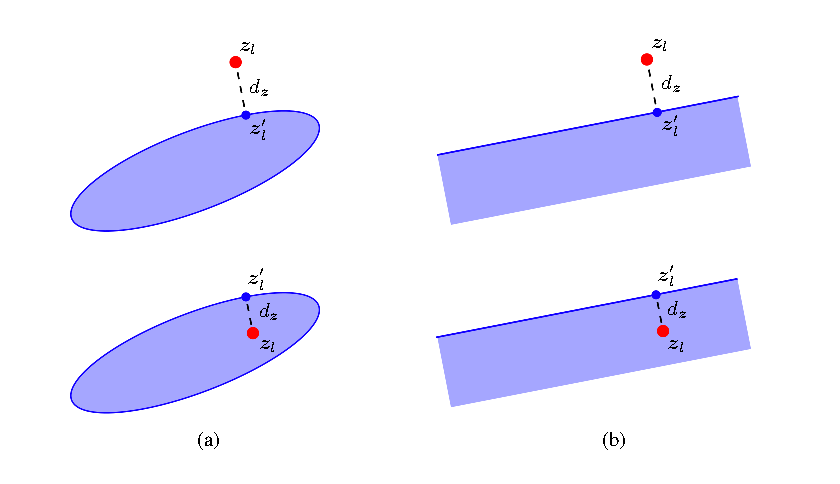
\includegraphics[scale=1]{./Figures/likelihoodApproximation.pdf}
\vspace{-5mm}
\caption{Graphical representation of the approximation used to obtain a closed form expression for $f(\V{z}_{l} | \V{x}_{k}, \V{e}_{k})$.}
\label{fig:likelihoodApproximation}
\end{figure*}

The likelihood function $f(\V{z}_{l} | \V{x}_{k}, \V{e}_{k})$ can be expressed as
\begin{align}
f(\V{z}_{l} | \V{x}_{k}, \V{e}_{k}) &= \int \rmv\rmv  f\big(\V{z}_{l} | \V{x}_{k}, \V{v}^{(l)}_k\big) \ist f\big(\V{v}^{(l)}_k| \V{e}_{k}\big) \ist  \mathrm{d} \V{v}^{(l)}_k \nn\\[.5mm]
%&= \frac{1}{|\Set{S}(\M{E}_{k})|} \int_{\Set{S}(\M{E}_{k})} \rmv\rmv \rmv\rmv \rmv\rmv  \mathcal{N}(\V{z}_{l} ;\V{p}_{k} \rmv+\rmv \V{v}^{(l)}_{k},\M{\Sigma}_{\V{u}_{l}}) \ist \mathrm{d} \V{v}^{(l)}_k \nn \\
&= \frac{1}{|\Set{S}(\M{E}_{k})|} \int_{\Set{S}(\M{E}_{k})} \rmv\rmv \rmv\rmv  \rmv\rmv  \mathcal{N}(\V{p}_{k} \rmv+\rmv \V{v}^{(l)}_{k};\V{z}_{l},\M{\Sigma}_{\V{u}_{l}} ) \ist \mathrm{d} \V{v}^{(l)}_k \label{eq:likelihoodInt}
\end{align}
where $|\Set{S}(\M{E}_{k})|$ is the surface or volume of $\Set{S}(\M{E}_{k})$. Let $\Set{S}_{\V{p}_{k}}\rmv\rmv(\M{E}_{k})$ be the area or surface $\Set{S}(\M{E}_{k})$ shifted by position $\V{p}_{k}$. With this notation, we can rewrite \eqref{eq:likelihoodInt} as
\begin{align}
f(\V{z}_{l} | \V{x}_{k}, \V{e}_{k}) &= \frac{1}{| \Set{S}(\M{E}_{k}) |} \int_{\Set{S}_{\V{p}_{k}}\rmv\rmv(\M{E}_{k})} \rmv\rmv \rmv\rmv  \rmv\rmv  \mathcal{N}(\V{v}^{(l)}_{k};\V{z}_{l},\M{\Sigma}_{\V{u}_{l}} ) \ist \mathrm{d} \V{v}^{(l)}_k. \label{eq:likelihoodInt2}
\end{align}
To obtain an approximate closed form expression for \eqref{eq:likelihoodInt}, we first introduce the point $\V{z}'_{l}$ on the boundary of $\Set{S}_{\V{p}_{k}}(\M{E}_{k})$ which is closest to the measurement $\V{z}_{l}$. This is shown in Fig.~\ref{fig:likelihoodApproximation}(a). Next, we also introduce the unit vector $\V{1}_{\V{z}_{l}} =  \frac{(\V{z}_{l} - \V{z}'_{l} )}{ \| \V{z}_{l} - \V{z}'_{l} \|}$ pointing from $\V{z}'_{l}$ to $\V{z}_{l}$ as well as the distance $d_{\V{z}_{l}} =  \| \V{z}_{l} - \V{z}'_{l} \|$  between $\V{z}'_{l}$ and $\V{z}_{l}$. By projecting $\RV{u}_{l}$ onto $\V{1}_{\V{z}_{l}}$, the scalar measurement noise $\rv{u}_{l}$ ``in the direction of $\V{z}_{l}$'' is obtained, i.e., $\rv{u}_{l} \sim \mathcal{N}\big(u_{l} ;0,\sigma^2_{u_{l}}\big)$ with $\sigma^2_{u_{l}} = \V{1}^{\mathrm{T}}_{\V{z}_{l}} \M{\Sigma}_{\V{u_l}} \V{1}_{\V{z}_{l}}$. 

%e the distance $d_{\V{z}_{l}} = \| \V{z}_{l} - \V{p}_{k} \| $  of observed measurement $\V{z}_{l}$ to object position $\V{p}_{k}$ and t
We now assume that the extent of the object is much larger than the measurement noise standard deviation  $\sigma_{u_{l}}$ and approximate the extent of the object by an infinite plane or volume. This approximation is shown in Fig.~\ref{fig:likelihoodApproximation}(b). Based on this approximation it is now straightforward to see that the high-dimensional integration in \eqref{eq:likelihoodInt2} can be replaced by the following one-dimensional\vspace{1mm} integrations
\begin{align}
 &f(\V{z}_{l} | \V{x}_{k}, \V{e}_{k}) \approx  \begin{cases}
   \frac{1}{| \Set{S}(\M{E}_{k}) |}  \int_{d_{\V{z}_l}}^{\infty} \hspace{2mm} \mathcal{N}(v^{(l)}_{k};0,\sigma^2_{u_{l}}) \ist \mathrm{d} v^{(l)}_k  \ist, &  \V{z}_l \notin \Set{S}_{\V{p}_{k}}\rmv\rmv(\M{E}_{k}) \\[1.5mm]
    \frac{1}{| \Set{S}(\M{E}_{k}) |}  \int^{\infty}_{-d_{\V{z}_l}}  \mathcal{N}(v^{(l)}_{k};0,\sigma^2_{u_{l}} ) \ist \mathrm{d} v^{(l)}_k   \ist, & \V{z}_l \in \Set{S}_{\V{p}_{k}}\rmv\rmv(\M{E}_{k})  . 
   \end{cases} \label{eq:likelihoodApproximation1D} \\[-6mm]
   \nn
\end{align}
A closed-form expression for the integrations in \eqref{eq:likelihoodApproximation1D} can be obtained by means of the Q-function \cite{BorSun:J79}, i.e.,
\begin{align}
 &f(\V{z}_{l} | \V{x}_{k}, \V{e}_{k}) \approx  \begin{cases}
   \frac{1}{| \Set{S}(\M{E}_{k}) |} \ist\ist Q\Big(\frac{\phantom{-}d_{\V{z}_l}}{\sigma_{u_{l}}}\Big), &  \V{z}_l \notin \Set{S}_{\V{p}_{k}}\rmv\rmv(\M{E}_{k}) \\[1.5mm]
    \frac{1}{| \Set{S}(\M{E}_{k}) |} \ist\ist  Q\Big(\frac{-d_{\V{z}_l}}{\sigma_{u_{l}}}\Big), & \V{z}_l \in \Set{S}_{\V{p}_{k}}\rmv\rmv(\M{E}_{k}) . 
   \end{cases} \label{eq:likelihoodApproximation1DQ} \\[-6.5mm]
   \nn
\end{align}

In addition, we discuss an important special case where $f(\V{z}_{l} | \V{x}_{k}, \V{e}_{k})$ can be evaluated by avoiding any approximation. Let us assume the measurement noise is iid, i.e., $\RV{u}_{l} \sim \mathcal{N}\big(\V{u}_{l} ;0,\sigma^2_{u_{l}} \M{I}\big)$. Furthermore, $\V{v}_l$ is uniformly distributed on a support $\Set{S}_{\mathrm{c}}(\M{E}_{k})$ that has the shape of a rectangle or cube. For a 3-D scenario, we recall that the eigenvalues and  eigenvectors of $\M{E}_{k}$ that define dimension and orientation of the cube, are denoted as $\lambda_{1,\M{E}_{k,n}} > \lambda_{2,\M{E}_{k,n}} > \lambda_{3,\M{E}_{k,n}} \geq 0$ as well as  $\protect\V{\lambda}_{1,\M{E}_{k,n}}$, $\protect\V{\lambda}_{2,\M{E}_{k,n}}$, and $\protect\V{\lambda}_{3,\M{E}_{k,n}}$, respectively.  Let $\Set{S}_{\V{p}_{k}}\rmv\rmv(\M{E}_{k})$ be the cube $\Set{S}_{\mathrm{c}}(\M{E}_{k})$ shifted by position $\V{p}_{k}$. In addition, let $d^{(1)}_{1,\V{z}_l}$ and $d^{(2)}_{1,\V{z}_l}$ be the distances of the measurement $\V{z}_l$ to the two parallel edges of the cube $\Set{S}_{\V{p}_{k}}\rmv\rmv(\M{E}_{k})$ defined by dimension $\lambda_{1,\M{E}_{k,n}}$ and axis $\V{\lambda}_{1,\M{E}_{k,n}}\rmv$. The likelihood contribution $\mathpzc{f}_1(\V{z}_{l} | \V{x}_{k}, \V{e}_{k})$ ``along direction $\lambda_{1,\M{E}_{k,n}}\rmv\rmv$'' can now be written\vspace{0mm} as 
\begin{align}
 &\mathpzc{f}_1(\V{z}_{l} | \V{x}_{k}, \V{e}_{k}) =  \begin{cases}
   1- \int^{\infty}_{d^{(2)}_{1,\V{z}_l}}  \mathcal{N}(v^{(l)}_{k};0,\sigma^2_{u_{l}} ) \ist \mathrm{d} v^{(l)}_k - \int^{\infty}_{d^{(1)}_{1,\V{z}_l}}  \mathcal{N}(v^{(l)}_{k};0,\sigma^2_{u_{l}} ) \ist \mathrm{d} v^{(l)}_k, &  \quad \lambda_{1,\M{E}_{k,n}} > d^{(1)}_{1,\V{z}_l}, d^{(2)}_{1,\V{z}_l} \\[3mm]
  \hspace{6.5mm}  \int^{\infty}_{d^{(1)}_{1,\V{z}_l}}  \mathcal{N}(v^{(l)}_{k};0,\sigma^2_{u_{l}} ) \ist \mathrm{d} v^{(l)}_k - \int^{\infty}_{d^{(2)}_{1,\V{z}_l}}  \mathcal{N}(v^{(l)}_{k};0,\sigma^2_{u_{l}} ) \ist \mathrm{d} v^{(l)}_k, & \quad d^{(2)}_{1,\V{z}_l} \geq \lambda_{1,\M{E}_{k,n}}, d^{(1)}_{1,\V{z}_l} \\[3mm]
     \hspace{6.5mm} \int^{\infty}_{d^{(2)}_{1,\V{z}_l}}  \mathcal{N}(v^{(l)}_{k};0,\sigma^2_{u_{l}} ) \ist \mathrm{d} v^{(l)}_k - \int^{\infty}_{d^{(1)}_{1,\V{z}_l}}  \mathcal{N}(v^{(l)}_{k};0,\sigma^2_{u_{l}} ) \ist  \mathrm{d} v^{(l)}_k, & \quad d^{(1)}_{1,\V{z}_l} \geq  \lambda_{1,\M{E}_{k,n}}, d^{(2)}_{1,\V{z}_l}. \nn
   \end{cases} \\[-1mm]
   \label{eq:likelihood3D}  \\[-8mm]
   \nn
\end{align}
Here, the first line is the probability that $\V{z}_l$ is located between the two edges along direction $\lambda_{1,\M{E}_{k,n}}$ and lines 2 and 3 are the probabilities that $\V{z}_l$ is not located between the two edges and closer to edge one or closer to edge two, respectively. A closed-form expression for the integrations in \eqref{eq:likelihood3D} can again be obtained by means of the Q-function\vspace{-4mm}, i.e.,
\begin{align}
 &\mathpzc{f}_1(\V{z}_{l} | \V{x}_{k}, \V{e}_{k}) =  \begin{cases}
   1- Q\bigg(\frac{d^{(1)}_{1,\V{z}_l}}{\sigma_{u_{l}}}\bigg) - Q\bigg(\frac{d^{(2)}_{1,\V{z}_l}}{\sigma_{u_{l}}}\bigg), &  \lambda_{1,\M{E}_{k,n}} > d^{(1)}_{1,\V{z}_l}, d^{(2)}_{1,\V{z}_l} \\[3mm]
   Q\bigg(\frac{d^{(1)}_{1,\V{z}_l}}{\sigma_{u_{l}}}\bigg) - Q\bigg(\frac{d^{(2)}_{1,\V{z}_l}}{\sigma_{u_{l}}}\bigg), & d^{(2)}_{1,\V{z}_l} \geq \lambda_{1,\M{E}_{k,n}}, d^{(1)}_{1,\V{z}_l}\\[3mm]
   Q\bigg(\frac{d^{(2)}_{1,\V{z}_l}}{\sigma_{u_{l}}}\bigg) - Q\bigg(\frac{d^{(1)}_{1,\V{z}_l}}{\sigma_{u_{l}}}\bigg), & d^{(1)}_{1,\V{z}_l} \geq  \lambda_{1,\M{E}_{k,n}}, d^{(2)}_{1,\V{z}_l}. \nn
   \end{cases}\nn \\[-5mm]
   \nn
\end{align}

Now, we can introduce $\mathpzc{f}_2(\V{z}_{l} | \V{x}_{k}, \V{e}_{k})$ and $\mathpzc{f}_3(\V{z}_{l} | \V{x}_{k}, \V{e}_{k})$ based on remaining eigenvalues $\lambda_{2,\M{E}_{k,n}}$, $\lambda_{3,\M{E}_{k,n}}$ and eigenvectors $\V{\lambda}_{2,\M{E}_{k,n}}$, $\V{\lambda}_{3,\M{E}_{k,n}}$ of $\M{E}_{k,n}$. The final closed form of the likelihood function for the case where $\V{v}_l$ is uniformly distributed on cube $\Set{S}_{\mathrm{c}}(\M{E}_{k})$ and the measurement noise $\V{u}_l$ is iid Gaussian, then reads
\begin{align}
f(\V{z}_{l} | \V{x}_{k}, \V{e}_{k})  = \frac{1}{| \Set{S}_{\mathrm{c}}(\M{E}_{k}) |} \ist\ist \mathpzc{f}_1(\V{z}_{l} | \V{x}_{k}, \V{e}_{k}) \ist\ist \mathpzc{f}_2(\V{z}_{l} | \V{x}_{k}, \V{e}_{k}) \ist\ist \mathpzc{f}_3(\V{z}_{l} | \V{x}_{k}, \V{e}_{k}). \nn\\[-7mm]
\nn
 \end{align}

\section{Implementation of the Proposed EOT Method}
Pseudocode for one time step of the proposed EOT method is provided in Algorithm~\ref{al:totalEOT1}. This pseudocode closely follows the presentation of the particle-based implementation discussed in \cite[Section~V]{MeyWil:J21}. MATLAB code is available on \texttt{fmeyer.ucsd.edu}.


\vspace{-5mm}
\begin{algorithm}
\SetAlgoLined
\tiny
\vspace{.8mm}

$\bigg[\Big\{  \big\{ \big( \V{x}^{(j)}_{k}\rmv\rmv, \V{e}^{(j)}_{k}\rmv\rmv, w^{(j)}_{k} \big) \big\}_{j=1}^{J} \Big\}_{k=1}^{\underline{K} +M} \bigg]= \text{EOT}\Big[ \Big\{  \big\{ \big( \V{x}^{-(j)}_{k}\rmv\rmv, \V{e}^{-(j)}_{k}\rmv\rmv, w^{-(j)}_{k} \big) \big\}_{j=1}^{J} \Big\}_{k=1}^{\underline{K}}\rmv, \big\{\V{z}_l \big\}_{l=1}^{M} \Big]$\\
\vspace{1mm}



\For{$k = 1 : \underline{K}$}{ \hspace{120mm} \bl{\tcp{\tiny prediction for legacy POs}}
\vspace{-1mm}
  \For{$j = 1 : J$}{
  \vspace{-.8mm}
     Compute $\underline{w}^{(1,j)}_{k} \rmv= p_{\mathrm{s}} \ist\ist \mathpzc{e}^{-\mu_{\mathrm{m}}\big(\underline{\V{x}}^{(j)}_{k}\rmv, \ist\underline{\V{e}}^{(j)}_{k}\big)} \ist w^{-(j)}_{k}$ and set $\underline{w}^{(1,j)}_{kl} \rmv\triangleq \underline{w}^{(1,j)}_{k}\rmv, l \rmv\in\rmv \{1,\dots,M\}$ 
  } 
  Calculate $p^{-\text{e}}_{k} = \sum^{J}_{j=1} w^{-(j)}_{k}$; $\tilde{\underline{\alpha}}^{\mathrm{n}}_k = \big(1-p^{-\text{e}}_{k}\big) + \big(1\!-\rmv p_{\ist\mathrm{s}}\big) p^{-\text{e}}_{k}$; and $\tilde{\underline{\alpha}}_k = \sum^{J}_{j\rmv=\rmv1} \underline{w}^{(1,j)}_{k} + \tilde{\underline{\alpha}}^{\mathrm{n}}_k$ \\[.5mm]
  Set $\tilde{\underline{\alpha}}^{\mathrm{n}(p)}_{kl}  \triangleq \tilde{\underline{\alpha}}^{\mathrm{n}}_k $, $l \rmv\in\rmv \{1,\dots,M\}$ and $\tilde{\underline{\alpha}}^{(p)}_{kl}  \triangleq \tilde{\underline{\alpha}}_k $, $l \rmv\in\rmv \{1,\dots,M\}$
}
\vspace{1mm}

\For{$k = 1 : M$}{ \hspace{120mm} \bl{\tcp{\tiny initialization of new POs}}
\vspace{-1mm}
    \For{$j = 1 : J$}{ 
      Draw $\Big(\overline{\boldsymbol{x}}_k^{(j)}\rmv\rmv, \overline{\boldsymbol{e}}_k^{(j)} \Big) \sim f_{\mathrm{p}} \rmv\big(\overline{\boldsymbol{x}}_k,\overline{\boldsymbol{e}}_k;\V{z}_k\big)$,
      compute $\overline{w}^{(1,j)}_{k} \rmv= \frac{q \rmv\Big(\overline{\boldsymbol{x}}_k^{(j)}\rmv\rmv, \overline{\boldsymbol{e}}_k^{(j)}\rmv\rmv, \overline{r}_k = 1 \Big)}{f_{\mathrm{p}} \rmv\Big(\overline{\boldsymbol{x}}_k^{(j)}\rmv\rmv, \overline{\boldsymbol{e}}_k^{(j)};\V{z}_l\Big)}$, and set $\overline{w}^{(1,j)}_{kl} \rmv\triangleq \overline{w}^{(1,j)}_{k}\rmv, l \rmv\in\rmv \{k,\dots,M\}$ 
    } 
  Calculate $\tilde{\overline{\alpha}}_k = \sum^{J}_{j\rmv=\rmv1} \overline{w}^{(1,j)}_{k} + 1$ \\[.5mm]
    Set $\tilde{\overline{\alpha}}^{\hspace{.1mm}\mathrm{n}(1)}_{kl}  \triangleq 1$, $l \rmv\in\rmv \{k\dots M\}$ and $\tilde{\overline{\alpha}}^{(1)}_{kl}  \triangleq \tilde{\overline{\alpha}}_k $, $l \rmv\in\rmv \{k\dots M\}$
}
\vspace{1mm}

\For{$p = 1 : P$}{
\vspace{1mm}

\For{$k = 1 : \underline{K}$}{ \hspace{89mm} \bl{\tcp{\tiny perform measurement evaluation for legacy POs}}
\vspace{-2mm}
  \For{$l = 1 : M$}{
  \vspace{1mm}
    Calculate $\tilde{\underline{\beta}}_{kl}^{(p)} = \frac{1}{\mu_{\mathrm{fa}} \ist f_{\mathrm{fa}}(\V{z}_{l}) \ist \tilde{\underline{\alpha}}_{kl}^{(p)} } \hspace{.5mm} \sum^{J}_{j=1} \underline{w}^{(p,j)}_{kl} \mu_{\mathrm{m}}\Big(\underline{\V{x}}^{(j)}_k,\underline{\V{e}}^{(j)}_k\Big) \ist f\Big(\V{z}_{l}| \underline{\V{x}}^{(j)}_k, \underline{\V{e}}^{(j)}_{k}\Big)$ 
      } 
}
\vspace{1.5mm}

\For{$k = 1 : M$}{\hspace{93mm} \bl{\tcp{\tiny perform measurement evaluation for new POs}}
\vspace{-1.5mm}
Compute $\tilde{\overline{\beta}}_{kk}^{(p)} = \frac{1}{\mu_{\mathrm{fa}} \ist f_{\mathrm{fa}}(\V{z}_{k}) \ist \tilde{\overline{\alpha}}_{kk}^{\hspace{.15mm}\mathrm{n}(p)} } \hspace{.5mm} \sum^{J}_{j=1}  \overline{w}^{(p,j)}_{kk} \mu_{\mathrm{m}}\Big(\overline{\V{x}}^{(j)}_k\rmv,\overline{\V{e}}^{(j)}_k\Big) \ist f\Big(\V{z}_{l}| \overline{\V{x}}^{(j)}_k\rmv, \overline{\V{e}}^{(j)}_{k}\Big)$
 \vspace{1.5mm}
 
  \For{$l = k\rmv+\rmv1 : M$}{
  \vspace{1mm}
    Calculate $\tilde{\overline{\beta}}_{kl}^{(p)} = \frac{1}{\mu_{\mathrm{fa}} \ist f_{\mathrm{fa}}(\V{z}_{l}) \ist \tilde{\overline{\alpha}}_{kl}^{(p)} } \hspace{.5mm} \sum^{J}_{j=1}  \overline{w}^{(p,j)}_{kl} \mu_{\mathrm{m}}\Big(\overline{\V{x}}^{(j)}_k,\overline{\V{e}}^{(j)}_k \Big) \ist f\Big(\V{z}_{l}| \overline{\V{x}}^{(j)}_k, \overline{\V{e}}^{(j)}_{k}\Big)$  } 
}
\vspace{1mm}

\For{$k = 1 : \underline{K}$}{  \hspace{74mm} \bl{\tcp{\tiny combine measurement evaluation information for legacy POs}}
\vspace{-1mm}

    Compute $\tilde{\underline{\xi}}_{kl}^{(p)} \triangleq \sum^{\underline{K}}_{\substack{k'=1\\k' \neq k}} \ist \tilde{\underline{\beta}}_{k'l}^{(p)} + \sum^{l}_{\substack{\ell=1}} \ist \tilde{\overline{\beta}}_{\ell l}^{(p)} + 1$
}
\vspace{1mm}

\For{$k = 1 : M$}{  \hspace{78mm} \bl{\tcp{\tiny combine measurement evaluation information for new POs}}
\vspace{-1mm}

Calculate $\tilde{\overline{\xi}}_{kl}^{(p)} \triangleq \sum^{\underline{K}}_{\substack{k'=1}} \ist \tilde{\underline{\beta}}_{k'l}^{(p)} + \sum^{l}_{\substack{\ell=1\\[.5mm] \ell \neq k}} \ist \tilde{\overline{\beta}}_{\ell l}^{(p)} + 1$
}
\vspace{1mm}


\If{$p < P$}{ \hspace{66.5mm} \bl{\tcp{\tiny calculate extrinsic information messages for legacy and new POs}}
\vspace{-2mm}
\For{$k = 1 : \underline{K}$}{
\For{$l = 1 : M$}{
Compute $\underline{w}^{(p\hspace{.1mm}+\hspace{.1mm}1,j)}_{kl} =\ist \underline{w}^{(1,j)}_{k} \hspace{.5mm} \prod^{M}_{\substack{l'=1\\l' \neq l}} \rmv\rmv \Bigg(  \frac{\mu_{\mathrm{m}}\Big(\underline{\V{x}}^{(j)}_{k}\rmv\rmv,\underline{\V{e}}^{(j)}_{k}\Big) f\Big(\V{z}_{l'}| \underline{\V{x}}^{(j)}_k\rmv\rmv, \underline{\V{e}}^{(j)}_{k}\Big)}{\mu_{\mathrm{fa}}  f_{\mathrm{fa}}\big(\V{z}_{l'}\big)} \ist + \ist \tilde{\underline{\xi}}_{kl'}^{(p)} \rmv \Bigg)$ \\[1.2mm]

Calculate $\tilde{\underline{\alpha}}^{\mathrm{n}(p+1)}_{kl}  =\ist \tilde{\underline{\alpha}}^{\mathrm{n}}_k \hspace{.5mm} \prod^{M}_{\substack{l'=1\\l' \neq l}}  \tilde{\underline{\xi}}_{kl'}^{(p)}$ and $\tilde{\underline{\alpha}}^{(p+1)}_{kl} = \sum^{J}_{j\rmv=\rmv1} \underline{w}^{(p+1,j)}_{kl} + \tilde{\underline{\alpha}}^{\mathrm{n}(p+1)}_{kl} $
}
}

\For{$k = 1 : M$}{
\For{$l = k : M$}{
Compute $\overline{w}^{(p\hspace{.1mm}+\hspace{.1mm}1,j)}_{kl} =\ist \overline{w}^{(1,j)}_{k} \frac{\mu_{\mathrm{m}}\Big(\overline{\V{x}}^{(j)}_{k}\rmv\rmv,\overline{\V{e}}^{(j)}_{k}\Big) f\Big(\V{z}_{k}| \overline{\V{x}}^{(j)}_k\rmv\rmv, \overline{\V{e}}^{(j)}_{k}\Big)}{\mu_{\mathrm{fa}}  f_{\mathrm{fa}}\big(\V{z}_{k}\big)} \hspace{.5mm} \prod^{M}_{\substack{l'=k+1\\l' \neq l}} \rmv\rmv \Bigg(  \frac{\mu_{\mathrm{m}}\Big(\overline{\V{x}}^{(j)}_{k}\rmv\rmv,\overline{\V{e}}^{(j)}_{k}\Big) f\Big(\V{z}_{l'}| \overline{\V{x}}^{(j)}_k\rmv\rmv, \overline{\V{e}}^{(j)}_{k}\Big)}{\mu_{\mathrm{fa}}  f_{\mathrm{fa}}\big(\V{z}_{l'}\big)} \ist + \ist \tilde{\overline{\xi}}_{kl'}^{(p)} \rmv \Bigg)$ \\[1.2mm]

Calculate $\tilde{\overline{\alpha}}^{\hspace{.1mm}\mathrm{n}(p+1)}_{kl}  =\ist \tilde{\overline{\alpha}}^{\mathrm{n}}_k \hspace{.5mm} \prod^{M}_{\substack{l'=k\\l' \neq l}} \rmv \tilde{\overline{\xi}}_{kl'}^{(p)}$ and $\tilde{\overline{\alpha}}^{(p+1)}_{kl} = \sum^{J}_{j\rmv=\rmv1} \overline{w}^{(p+1,j)}_{kl} + \tilde{\overline{\alpha}}^{\hspace{.1mm}\mathrm{n}(p+1)}_{kl} $
}
}
}
\vspace{1mm}

\If{$p = P$}{ \hspace{95.3mm} \bl{\tcp{\tiny calculate beliefs for legacy and new POs}}
\vspace{-2mm}

\For{$k = 1 : \underline{K}$}{
Compute $\underline{w}^{\text{A}(j)}_{k} =\ist \underline{w}^{(1,j)}_{k} \hspace{.5mm} \prod^{M}_{\substack{l=1}} \rmv\rmv \Bigg(  \frac{\mu_{\mathrm{m}}\Big(\underline{\V{x}}^{(j)}_{k}\rmv\rmv,\underline{\V{e}}^{(j)}_{k}\Big) f\Big(\V{z}_{l}| \underline{\V{x}}^{(j)}_k\rmv\rmv, \underline{\V{e}}^{(j)}_{k}\Big)}{\mu_{\mathrm{fa}}  f_{\mathrm{fa}}\big(\V{z}_{l}\big)} \ist + \ist \tilde{\underline{\xi}}_{kl}^{(P)} \rmv \Bigg)$ and $\underline{w}^{\text{B}}_{k} =\ist \tilde{\underline{\alpha}}^{\mathrm{n}}_k \hspace{.8mm} \prod^{M}_{\substack{l=1}}  \tilde{\underline{\xi}}_{kl}^{(P)}$ \\[0mm]

Calculate $\underline{w}^{(j)}_{k} \ist=\ist \frac{\underline{w}^{\text{A}(j)}_{k}}{\underline{w}^{\text{B}}_{k}+\sum^{J}_{j'=1} \ist \underline{w}^{\text{A}(j')}_{k}}$
}

\For{$k = 1 : M$}{ \hspace{93mm} 
\vspace{-1mm}

Compute $\overline{w}^{\hspace{.1mm}\text{A}(j)}_{k} =\ist \overline{w}^{(1,j)}_{k} \ist \frac{\mu_{\mathrm{m}}\Big(\overline{\V{x}}^{(j)}_{k}\rmv\rmv,\overline{\V{e}}^{(j)}_{k}\Big) f\Big(\V{z}_{k}| \overline{\V{x}}^{(j)}_k\rmv\rmv, \overline{\V{e}}^{(j)}_{k}\Big)}{\mu_{\mathrm{fa}}  f_{\mathrm{fa}}\big(\V{z}_{k}\big)} \hspace{.7mm} \prod^{M}_{\substack{l=k+1}} \rmv\rmv \Bigg(  \frac{\mu_{\mathrm{m}}\Big(\overline{\V{x}}^{(j)}_{k}\rmv\rmv,\overline{\V{e}}^{(j)}_{k}\Big) f\Big(\V{z}_{l}| \overline{\V{x}}^{(j)}_k\rmv\rmv, \overline{\V{e}}^{(j)}_{k}\Big)}{\mu_{\mathrm{fa}}  f_{\mathrm{fa}}\big(\V{z}_{l}\big)} \ist + \ist \tilde{\overline{\xi}}_{kl}^{(P)} \rmv \Bigg)$ and $\overline{w}^{\text{B}}_{k} =\ist \tilde{\overline{\alpha}}^{\mathrm{n}}_k \hspace{.8mm} \prod^{M}_{\substack{l=k}}  \tilde{\overline{\xi}}_{kl}^{(P)}$ \\[0mm]

Calculate $\overline{w}^{(j)}_{k} \ist=\ist \frac{\overline{w}^{\hspace{.15mm}\text{A}(j)}_{k}}{\overline{w}^{\text{B}}_{k}+\sum^{J}_{j'=1} \ist \overline{w}^{\hspace{.15mm}\text{A}(j')}_{k}}$
}

}
\vspace{1mm}

}
\vspace{1mm}

Output: $\Big\{  \big\{ \big( \V{x}^{(j)}_{k}\rmv\rmv, \V{e}^{(j)}_{k}\rmv\rmv, w^{(j)}_{k} \big) \big\}_{j=1}^{J} \Big\}_{k=1}^{\underline{K} +M}$

\caption{Proposed Particle-Based EOT Method --- Single Time Step}
\label{al:totalEOT1}
\end{algorithm}

\pagebreak



\bibliographystyle{IEEEtran}
\bibliography{IEEEabrv,StringDefinitions,Books,Papers,Temp}



\end{document}
%%%%%%%%%%%%%%%%%%%%%%%%%%%%%%%%%%%%%%%%%%%%%%%%%%%%%%%%%%%%%%%%%%%%%%%%%%%%%%%%
